\documentclass[12pt, a4paper, twoside, openany]{book}
\usepackage[
    a4paper, 
    total={6in, 8in}, 
    top=2cm,
    left=3cm,
    right=2.5cm,
    bottom=1.25cm,
    includeheadfoot,
    headheight=40pt,
]{geometry}
\usepackage[T1]{polski}
\usepackage{graphicx}
\usepackage{fancyhdr}
\usepackage{mathptmx}
\usepackage{enumitem}
\usepackage[utf8]{inputenc}
\usepackage{import}
\usepackage{setspace}
\usepackage{titlesec}
\usepackage{multirow}
\usepackage{longtable}
\usepackage{url}
\usepackage{tabularray}
\usepackage{float}
\usepackage{listings}
\usepackage{calc}
\usepackage{rotating}

\import{../}{commands.tex}

\fancypagestyle{plain}{
    \fancyhf{}
    \renewcommand{\headrulewidth}{0pt}
    \fancyhead[C]{\uniimage}
    \fancyfoot[LE,RO]{\thepage}
}

\newlength\imgth
\setlength\imgth{\textwidth}
\addtolength\imgth{-0.3\textwidth}

\newlength\fittingimage
\setlength\fittingimage{\textheight}
\addtolength\fittingimage{-0.15\textheight}

% Wymogi edycyjne: https://moodle2.e-wsb.pl/pluginfile.php/7505508/mod_resource/content/2/Wymogi%20edycyjne_praca%20dyplomowa.pdf

\NewTblrTheme{fancy}{
    \SetTblrStyle{firsthead}{foot=\bfseries}
    \SetTblrStyle{firstfoot}{fg=blue2}
    \SetTblrStyle{middlefoot}{\itshape}
    \SetTblrStyle{caption-tag}{red2}
}

\DefTblrTemplate{contfoot-text}{default}{}
\DefTblrTemplate{conthead-text}{default}{}
\DefTblrTemplate{conthead}{default}{}
\DefTblrTemplate{capcont}{default}{}

\newcommand{\forceindent}{\leavevmode{\parindent=1.3em\indent}}

\renewcommand\thesection{\Alph{chapter}\arabic{section}}

\addtolength{\topmargin}{-34.91641pt}

\linespread{1.5}

\setlist[itemize]{label=--}

\begin{document}

% Header & footer settings :)
\pagestyle{plain}

\titleformat
{\chapter} %/{〈command 〉}
[block] %/[〈shape〉]
{\bfseries\large} %/ {〈format〉}
{} %/ {〈label 〉}
{0.5ex} %/ {〈sep〉}
{
    \centering
} %/ {〈before-code〉}
{
    \vspace{-0.5ex}%
} %/ {〈after-code〉}

\setcounter{secnumdepth}{4}

\titleformat{\section}[hang]{\normalfont\bfseries}{\thesection.}{0.5em}{}

\titleformat{\subsection}[hang]{\normalfont\bfseries}{\thesubsection.}{0.4em}{}

\titleformat{\subsubsection}[hang]{\normalfont\bfseries}{\thesubsubsection.}{0.4em}{}

\begin{titlepage}
    \begin{center}

        \uniimage

        \MakeUppercase{\department}

        \vspace{5cm}

        \begin{Large} \textbf{Trashify – rozpoznawanie pojemników na odpady za pomocą algorytmów uczenia maszynowego} \end{Large}

        \vspace{5cm}

        PROJEKT DYPLOMOWY

        \vfill
        Poznań 2024

    \end{center}
\end{titlepage}

\setcounter{tocdepth}{3}

\chapter{\MakeUppercase{dane partnerów}}

\section{Dane Promotora}

\noindent
\begin{tabular}{ |p{5cm}|p{9cm}|}
    \hline
    Imię i nazwisko         & Izabela Janicka-Lipska \\
    \hline
    Stopień / Tytuł naukowy & dr inż.                \\
    \hline
    Data i podpis           &                        \\ \hline
\end{tabular}

\section{Dane członków Zespołu projektu}

\membersTable

% Example table and figure formatting
\section{Wprowadzenie}
\forceindent W dzisiejszym świecie, kiedy problem zanieczyszczenia środowiska staje się coraz bardziej palący, zarządzanie odpadami staje się kluczowym aspektem naszego życia. Statystyki nie pozostawiają złudzeń -- rosnąca produkcja odpadów na skalę globalną stawia przed nami istotne wyzwania. Na całym świecie rocznie wytwarza się ogromne ilości odpadów, z których część jest nadal nieefektywnie zagospodarowana, co prowadzi do negatywnego wpływu na środowisko naturalne. W samej Polsce, roczna produkcja odpadów na rok 2021 wyniosła 121 milionów ton, z czego 11.3\% stanowiły odpady komunalne. \footnote{S. 149; Główny Urząd Statystyczny -- Ochrona środowiska 2022, Warszawa, 2022r.}

Jednym z kluczowych aspektów tego wyzwania jest efektywne segregowanie i recykling odpadów, co przyczynia się nie tylko do ochrony środowiska naturalnego, ale także do potencjalnych oszczędności. Jak podaje EEA (Europejska Agencja Ochrony Środowiska), na obywatela Unii Europejskiej przypada średnio 4,8 ton odpadów komunalnych, z czego 49\% jest recyklingowanych \footnote{Dane za stroną internetową (dostęp: 03.11.2023r.) \url{https://www.eea.europa.eu/en/topics/in-depth/waste-and-recycling}}. Recykling może przynieść znaczące korzyści gospodarcze i środowiskowe, w tym zmniejszenie emisji gazów cieplarnianych, ograniczenie zużycia surowców naturalnych oraz tworzenie miejsc pracy. W samej Polsce, między latami 2004 i 2020, procent recyklingu odpadów komunalnych wzrósł z poziomu 4,9 do 38.7\%.

Jednakże, aby skutecznie promować segregację odpadów i recykling, niezbędne jest zrozumienie ludzkiego zachowania oraz eliminacja ,,tarcia`` związanego ze znalezieniem odpowiedniego pojemnika na odpady. Projekt oferujący łatwy dostęp do informacji o pojemnikach na odpady oraz lokalizacji najbliższego odpowiedniego kontenera usuwa bariery, które często zniechęcają do segregacji.

Niniejsza praca inżynierska skupia się na rozwiązaniu tego wyzwania poprzez wykorzystanie zaawansowanych technologii, takich jak sztuczna inteligencja, uczenie maszynowe, technologie wizyjne oraz geolokalizacja, w celu stworzenia systemu automatycznej klasyfikacji pojemników na odpady oraz aplikacji mobilnej, która umożliwia łatwiejsze lokalizowanie pojemników na śmieci w najbliższej okolicy. Naszym celem jest nie tylko zwiększenie efektywności gospodarki odpadami, ale także kształtowanie proekologicznego zachowania i eliminacja barier, które utrudniają segregację odpadów.

\chapter{\MakeUppercase{Założenia projektu}}

\section{Opis Projektu}

\subsection{Uzasadnienie wyboru tematu}

\forceindent Problem utylizacji odpadów stał się w ostatnich latach jednym z największych wyzwań dla społeczeństwa i środowiska naturalnego. Śmieci są produkowane w ogromnych ilościach, a nieprawidłowe postępowanie z nimi prowadzi do skażenia powietrza, wody i gleby. W związku z tym, istnieje potrzeba opracowania rozwiązań, które ułatwią zarządzanie odpadami w sposób bardziej skuteczny i zrównoważony.

Dzięki rozwojowi technologii uczenia maszynowego, pojawiła się możliwość stworzenia aplikacji mobilnej, która rozpoznawać będzie pojemniki na odpady na podstawie zdjęć oraz oznaczać je na mapie. Ułatwi ona lokalizowanie pojemników na dany typ odpadów oraz proces właściwego utylizowania śmieci dla użytkowników. Taka aplikacja może również zwiększyć świadomość społeczną w zakresie utylizacji odpadów i przyczynić się do zmniejszenia ilości odpadów zalegających na składowiskach.

Temat ten jest aktualny i ważny, a jednocześnie daje wiele możliwości na zastosowanie różnych technologii i algorytmów uczenia maszynowego. Przy realizacji projektu można wykorzystać m.in. sieci neuronowe, algorytmy uczenia głębokiego, przetwarzanie obrazów, uczenie maszynowe w chmurze oraz usługi geolokalizacyjne.

Podsumowując, projekt \topic jest uzasadniony ze względu na aktualność i ważność tematu, możliwość wykorzystania najnowszych technologii oraz potencjalne korzyści dla społeczeństwa i środowiska naturalnego.

\subsection{Problem badawczy}

\forceindent Problemem badawczym jest określenie algorytmów uczenia maszynowego najlepiej nadających się do rozpoznawania pojemników na odpady na podstawie zdjęć oraz określenie cech obrazów odpowiadających za skuteczność modelu.

W ramach tego problemu badawczego można skoncentrować się na kilku podproblemach, m.in.:
\begin{itemize}
    \item analiza dostępnych zbiorów danych:
          \begin{itemize}
              \item znalezienie zbiorów danych do treningu i testowania modelu rozpoznawania pojemników na odpady;
              \item określenie jak są one zdefiniowane oraz jakie informacje zawierają;
          \end{itemize}
    \item wybór odpowiednich algorytmów uczenia maszynowego:
          \begin{itemize}
              \item określenie algorytmów uczenia maszynowego, które najlepiej nadają się do rozpoznawania pojemników na odpady na podstawie zdjęć;
          \end{itemize}
    \item przygotowanie zbiorów danych:
          \begin{itemize}
              \item zastosowanie technik przetwarzania obrazów;
              \item potencjalne użycie technik augmentacji danych;
          \end{itemize}
    \item implementacja i trening modelu: wyłonienie najlepszej techniki trenowania modelu bazowanego na obrazach;
    \item ocena skuteczności modelu: określenie metryk, które pozwolą dokładnie ocenić skuteczność modelu w rozpoznawaniu pojemników na odpady;
    \item analiza cech obrazów: na podstawie analizy modelu, zlokalizowanie cech obrazów odpowiadających za skuteczność procesu rozpoznawania pojemników na odpady.
\end{itemize}

\subsection{Cel główny i cele szczegółowe projektu}

\forceindent Celem nadrzędnym jest stworzenie aplikacji mobilnej, która będzie pomagać użytkownikom w identyfikacji oraz lokalizowaniu pojemników na odpady danego typu. Aplikacja ta będzie miała na celu wspomaganie procesu utylizacji odpadów w odpowiedzialny i racjonalny sposób poprzez ułatwienie segregacji odpadów oraz zapobieganie ich niewłaściwemu składowaniu.

Cele podrzędne:
\begin{itemize}
    \item analiza dostępnych zbiorów danych: analiza zbiorów danych dostępnych w Internecie, które mogą posłużyć do treningu i testowania modelu rozpoznawania pojemników na odpady;
    \item wybór odpowiednich algorytmów uczenia maszynowego najlepiej nadających się do rozpoznawania pojemników na odpady na podstawie zdjęć;
    \item przygotowanie zbiorów danych do treningu modelu rozpoznawania pojemników na odpady;
    \item implementacja i trening modelu rozpoznawania pojemników na odpady;
    \item ocena skuteczności modelu rozpoznawania pojemników na odpady;
    \item analiza cech obrazów odpowiadających za skuteczność procesu rozpoznawania pojemników na odpady;
    \item określenie, które cechy obrazów mają największy wpływ na skuteczność procesu rozpoznawania i jak można je wykorzystać do dalszej optymalizacji modelu.
\end{itemize}

\subsection{Zakres podmiotowy, przedmiotowy, czasowy i przestrzenny}

\begin{itemize}
    \item Zakres podmiotowy projektu \topic  obejmuje opracowanie aplikacji mobilnej oraz badanie algorytmów uczenia maszynowego, które umożliwią rozpoznawanie pojemników na odpady. Podmiotem badania jest zatem użyteczność aplikacji mobilnej Trashify oraz modele uczenia maszynowego, które będą umożliwiać rozpoznawanie pojemników na odpady.
    \item Zakres przedmiotowy obejmuje badanie możliwości rozpoznawania różnych typów pojemników na odpady (np. pojemnik na papier, szkło, plastik, odpady organiczne itp.) oraz opracowanie algorytmów uczenia maszynowego, które umożliwią ich poprawną identyfikację. W ramach projektu będzie również opracowana aplikacja mobilna, która będzie integrować te algorytmy oraz udostępniać użytkownikom informacje o pojemnikach na odpady oraz umożliwiać im łatwe i szybkie ich zlokalizowanie.
    \item Zakres czasowy projektu obejmuje okres od 01.04.2023 aż do 01.12.2023.
    \item Zakres przestrzenny projektu obejmuje miejsce, w którym aplikacja Trashify będzie wykorzystywana, czyli przede wszystkim Polska. Projekt ogranicza się do konkretnego obszaru geograficznego, ponieważ algorytmy uczenia maszynowego, które zostaną opracowane w ramach projektu, będą skupiały się na pojemnikach na odpady spotykanych w Polsce. W ramach projektu nie będzie prowadzona analiza pojemników spotykanych w innych krajach.
\end{itemize}

\subsection{Metody i techniki badawcze}
\begin{itemize}
    \item Metoda analizy i konstrukcji logicznej:
          \begin{itemize}
              \item analiza składników aplikacji Trashify (np. interfejs użytkownika, algorytmy uczenia maszynowego, baza danych itp.);
              \item indywidualna analiza każdego z tych składników,
                    synteza wyników analizy w celu stworzenia spójnego i logicznego systemu informacyjnego.
          \end{itemize}
    \item Metoda statystyczna:
          \begin{itemize}
              \item badanie preferencji użytkowników w zakresie korzystania z aplikacji mobilnej Trashify na ograniczonej próbie;
              \item pozyskanie informacji o średniej ilości odpadów segregowanych przez użytkowników korzystających z aplikacji;
              \item analiza zależności pomiędzy poszczególnymi cechami użytkowników a ich zachowaniem w kontekście segregacji odpadów.
          \end{itemize}
    \item Metoda symulacji komputerowej:
          \begin{itemize}
              \item wykorzystanie algorytmów uczenia maszynowego do stworzenia modelu rozpoznającego typ pojemnika na odpady;
              \item przeprowadzenie symulacji na tym modelu, celem zbadania różnych czynników na jego dokładność (np. rozdzielczość zdjęcia, kąt pod jakim zostało ono wykonane, oświetlenie itp.).
          \end{itemize}
    \item Metoda heurystyczna:
          \begin{itemize}
              \item analiza problemów i wyzwań związanych z korzystaniem z aplikacji Trashify i sortowaniem odpadów przez użytkowników;
              \item odkrywanie nowych rozwiązań i podejść do tych problemów;
              \item badanie opinii użytkowników i na ich podstawie wprowadzanie ulepszeń w aplikacji.
          \end{itemize}
\end{itemize}

\section{Ryzyko związane z realizacją projektu}

\begin{enumerate}[label=--]
    \item Ryzyko technologiczne -- związane z wykorzystaniem nowych technologii, które mogą nie działać zgodnie z oczekiwaniami, bądź w trakcie projektowania i implementacji systemu, mogą pojawić się trudności techniczne.
    \item Ryzyko projektowe -- związane z niedostatecznymi planami, wyboru niewłaściwej metodyki lub zła interpretacja wymagań.
    \item Ryzyko jakościowe -- związane z niedostatecznymi testami, błędami w kodzie, które mogą prowadzić do awarii systemu, co może prowadzić do opóźnień w realizacji projektu.
    \item Ryzyko bezpieczeństwa -- związane z atakami cybernetycznymi na system, które mogą prowadzić do utraty danych lub przestojów w działaniu systemu.
\end{enumerate}

\chapter{Realizacja}

\section{Opracowanie projektu}

\subsection{Założenia teoretyczne}

\subsubsection{Interfejs aplikacji}

\forceindent \textbf{GraphQL}\\
\forceindent Opracowany przez firmę Facebook (obecnie Meta), Graphql jest językiem zapytań oraz środowiskiem wykonawczym do interakcji z danymi w aplikacjach, którego celem jest ograniczenie nadmiernego i niedostatecznego pobierania danych \footnote{S. 140; Gleison Brito, Thais Mombach, Marco Tulio Valente, Migrating to GraphQL: A Practical Assessment, ASERG Group, Department of Computer Science, Federal University of Minas Gerais, Brazil, 18.02.2019.}. Został zaprojektowany z myślą o urządzeniach mobilnych, biorąc pod uwagę ich niską prędkość, pamięć masową i drogie żądania internetowe.
W tym języku zapytań wszystkie żądania są wysyłane do pojedynczego punktu końcowego, a wykres danych, zwykle w formacie json, jest analizowany. Następnie zapytania są oceniane i stosowane są odpowiednie zapytania i mutacje.

Składa się on z głównych trzech części:
\begin{enumerate}
    \item Zapytań (ang. \textit{Queries}): Służą do pobierania danych z serwera. Klient definiuje, jakie informacje potrzebuje, a serwer dostarcza tylko te dane. \footnote{Dane za stroną internetową: \url{https://graphql.org/learn/queries/}, Rozdział ,,Queries and Mutations`` (dostęp: 12.11.2023r.)}
    \item Mutacji (ang. \textit{Mutations}): Pozwalają na modyfikację danych na serwerze, takie jak dodawanie, aktualizowanie lub usuwanie rekordów. \footnote{Dane za stroną internetową: \url{https://graphql.org/learn/queries/}, Rozdział ,,Queries and Mutations`` (dostęp: 12.11.2023r.)}
    \item Typów (ang. \textit{Types}): GraphQL definiuje struktury typów danych i relacje między nimi, co umożliwia klientowi zrozumienie, jakie dane mogą być dostępne i jakie zapytania można wykonywać.\footnote{Dane za stroną internetową: \url{https://graphql.org/learn/schema/}, Rozdział ,,Schemas and Types`` (dostęp: 12.11.2023r.)}
\end{enumerate}

\textbf{REST}\\
\forceindent REST to akronim REpresentational State Transfer\footnote{Rozdział 5; Roy Thomas Fielding, Architectural Styles and the Design of Network-based Software Architectures, 2000r.} i styl architektoniczny dla rozproszonych systemów hipermedialnych. Sam w sobie jest wzorcem architektonicznym, który zakłada rozdzielenie odpowiedzialności między zapytaniami (GET), mutacjami (POST, PATCH, PUT) i metodami usuwania (DELETE). Został on przetestowany w boju od 2000 roku i szeroko przyjęty w społeczności programistów.

\subsubsection{Warstwa komunikacji z bazą danych}
\subparagraph{Mapowanie obiektowo-relacyjne, mapowanie obiektowo-dokumentowe i budowniczy kwerend\\}
\forceindent  Mapery obiektowo-relacyjne, obiektowo-dokumentowe czy budowniczy kwerend są niezbędnymi narzędziami do utrzymywania deklaratywnego podejścia do komunikacji z systemem bazodanowym.
Na rynku dostępnych jest wiele bibliotek oferujących konkurujące rozwiązania.
Zespół postanowił zbadać możliwość wykorzystania każdej z kategorii abstrakcji, celem wyłonienia najbardziej dopasowanego do potrzeb rozwiązania.
Wybór ten determinuje ilość i złożoności kodu bazowego, a także wymagania techniczne dotyczące konfiguracji bazy danych.

\textbf{Mapowanie obiektowo-relacyjne\\}
\forceindent Wykorzystywanie mapowania obiektowo-relacyjnego (ang. \textit{Object Relational Mapping}) to powszechna praktyka w projektach programistycznych.
Stanowi ono dodatkową warstwę abstrakcji nad językiem SQL, czy budowniczym kwerend, zapewniając automatyczną konwersję obiektów źródłowych na ich odpowiedniki zrozumiałe dla bazy danych oraz rekordów bazodanowych na obiekty.
W kontekście baz danych, mapowanie obiektowo-relacyjne można uznać za najwyższą formę abstrakcji dla komunikacji z bazą danych w środowisku serwerowym.\footnote{S. 1-4; Alexandre Torres [i inni] Twenty years of object-relational mapping: A survey on patterns, solutions, and their implications on application design, 28.09.2016r.}

W środowisku node.js pojawiło się takowych wiele, między innymi:
\begin{enumerate}[label=--]
    \item TypeORM -- wykorzystujący eksperymentalne dekoratory w języku Typescript celem deklarowania schematu encji w bazie danych. Wszystkie operacje związane z językiem deklaracji danych są wykonywane przy ich użyciu.
    \item Sequelize -- najstarszy na tej liście maper obiektowo-relacyjny, pierwsze wzmianki o nim na witrynie StackOverflow sięgają roku 2011. Jest on dojrzałym, pełnym funkcjonalności maperem, którego popularność odzwierciedlona jest w 1,5 miliona tygodniowych pobrań\footnote{Dane za stroną internetową (dostęp 16.11.2023r.) \url{https://www.npmjs.com/package/sequelize}}.
    \item Prisma -- kontrowersyjny maper, którego operacje łączenia (ang. \textit{join}) wykonywane są w sposób wirtualny, to znaczy poprzez wysłanie kilku kwerend do bazy danych i połączeniu ich wedle instrukcji użytkownika w ,,Prisma Engine``, który napisany został przy pomocy języka Rust, co zapewnia relatywne bezpieczeństwo oraz wysoką wydajność takiego rozwiązania\footnote{Dane za stroną internetową (dostęp: 16.11.2023r.)\url{https://www.prisma.io/}}.
    \item Drizzle -- maper obiecujący pełne bezpieczeństwo typów ze składnią podobną do tej znanej z języka SQL oraz automatyczną generacją schematów za pomocą biblioteki Zod.
    \item Mikro-ORM -- oparty na domniemanych transakcjach, automatycznym grupowaniu kwerend za pomocą wzorca jednostki pracy (ang. \textit{Unit of Work}). Wzorowany jest na Hibernate, znanym z języka Java oraz Doctrine z PHP.\footnote{Dane za stroną internetową (dostęp: 16.11.2023r.) \url{https://mikro-orm.io/}}
\end{enumerate}

\newpage
\textbf{Mapowanie obiektowo-dokumentowe\\}
\forceindent Mapowanie obiektowo-dokumentowe powstało wraz z bazami NoSQL, których to system często nie posiada schematów danych.
Tak samo jak w przypadku mapowania obiektowo-relacyjnego, ma ono na celu uproszczenie interakcji pomiędzy aplikacją a bazą danych. Powstało ono w celu wyabstrakcjonowania procesu zarządzania i mapowania obiektów z ich natywnej dla bazy danych struktury, do takiej zrozumiałej przez język programowania, jak również utrzymującej konwencje programowania obiektowego.\footnote{S. 59130-59131; Alberto Hernandez Chillion [i inni], A Model-Driven Approach to Generate Schemas for Object-Document Mappers, IEEE Access, Murcja, Hiszpania}

W środowisku node.js na przestrzeni lat powstały między innymi następujące mapery obiektowo-dokumentowe:
\begin{enumerate}[label=--]
    \item mongoose -- dedykowany dla bazy MongoDB mapper obiektowo-dokumentowy. Posiada wiele funkcjonalności związane z procesem wzbogacania POJO (ang. \textit{plain-old-javascript-object}), ktore zapewniają walidację obiektów, dodawanie pól wirtualnych i inne.
    \item prisma -- maper obiektowo-relacyjny, posiadający wsparcie dla bazy MongoDB i funkcjonuje w trybie wymuszonej transakcyjności danych przy użyciu zbiorów replik (ang. \textit{replica set}).
\end{enumerate}

\textbf{Budowniczy kwerend\\}
\forceindent  Budowniczy kwerend stanowią abstrakcję na język SQL w wybranym języku programowania.
Pozwalają one na deklaratywne tworzenie kwerend za pomocą operacji takich jak: select, insert, join, delete, update, with, where, not, etc.
Zabezpieczają programistę przed niebezpieczeństwem literówek poprzez pełne wsparcie intellisense w danym języku programowania oraz rozwiązują popularne problemy związane z cyberbezpieczeństwem przeprowadzania operacji na bazie danych, czego najpopularniejszym przykładem są operacje wstrzykiwania SQL`a (ang. \textit{SQL Injection})\footnote{Tony Russell-Rose, Farhad Shokraneh, Designing the Structured Search Experience: Rethinking the Query-Builder Paradigm, Uniwersytet w Londynie, 2020r}.

\subsection{Typy baz danych}

\forceindent \textbf{Bazy nierelacyjne (NoSQL)}\\
\forceindent Bazy danych No-SQL nie mają tak sztywnego schematu bazy danych jak ich relacyjne odpowiedniki.
Struktura organizacyjna różni się w zależności od typu nierelacyjnej bazy danych\footnote{S.1; Deka Ganesha Chandra, BASE Analysis of NoSQL Database, Regional Vocational Training Instutite for Women, Tura, Meghalaya, India, 19.11.2012r.}.
Biorąc to pod uwagę, wszystkie mają na celu rozwiązanie problemów tradycyjnej, relacyjnej bazy danych, poprzez zaadresowanie kwestii elastyczności i skalowalności.
Bazy danych SQL nie są idealne do przechowywania nieustrukturyzowanych formatów danych, takich jak tekst, wideo i obrazy, co adresują bazy NoSQL.
Przedkładają one dostępność nad spójność.
Termin NoSQL nie oznacza, że dana baza danych nie obsługuje poleceń SQL, można go przetłumaczyć jako ,,nie tylko SQL``.

Rodzaje nierelacyjnych struktur baz danych to:
\begin{enumerate}[label=--]
    \item Key-value store -- jest to model bez schematu, w którym dane są zorganizowane w słownik par klucz-wartość.
          Klucz może być podobny do tego, jaki znajduje się w relacyjnej bazie danych, np. identyfikator koszyka, podczas gdy wartości są tablicą danych, np. każdy pojedynczy element w koszyku użytkownika.
          Są one powszechnie stosowane w systemach o dużej objętości, które wymagają najszybszego możliwego czasu reakcji.
          Ze względu na nieodłączną strukturę danych, nie są one dobrym rozwiązaniem, gdy potrzebne jest odzyskiwanie wielu rekordów na raz.
          Przykładami takich baz danych są Redis, Memcached, KeyDB, czy DragonflyDB\footnote{S. 5 -- 19; Marc Seeger, Key-Value stores: a practical overview, Computer Science and Media Ultra-Large-Sites SS09, Stuttgart, Germany, 21.09.2009r.}.
    \item Document store -- jak sama nazwa wskazuje, są to bazy danych, w których przechowywane są obiekty podobne do dokumentów.
          Dane przechowywane w takiej bazie danych są zwykle zorganizowane w formacie częściowo ustrukturyzowanym, takim jak JSON, XML lub BSON.
          Daje to programistom większą elastyczność, ponieważ schematy danych nie muszą dokładnie odpowiadać wzorcom innych dokumentów przechowywanych w danej kolekcji.
          Złożone transakcje mogą być jednak problematyczne i prowadzić do uszkodzenia danych.
          Popularne przypadki użycia dokumentowych baz danych obejmują systemy zarządzania treścią.
          Przykładem bazy danych zorientowanej na dokumenty jest MongoDB\footnote{S. 337; Robin Hecht, Stefan Jablonski, NoSQL Evaluation A Use Case Oriented Survey, International Conference on Cloud and Service Computing, 2011r.}.
    \item Wide-column store -- informacje są przechowywane w kolumnach, co pozwala użytkownikom uniknąć nadmiernego i niedostatecznego pobierania danych, ograniczając alokację pamięci.
          Ten typ bazy danych próbuje rozwiązać niedociągnięcia magazynów klucz-wartość i dokumentów, ale może być bardziej złożonym systemem do zarządzania, dlatego nie jest zalecana do stosowania w nowo powstałych projektach.
          Apache HBase i Apache Cassandra są przykładami baz danych o otwartym kodzie źródłowym i szerokim zakresie kolumn.
          Apache HBase jest zbudowany na bazie Hadoop Distributed Files System, który zapewnia sposób przechowywania rzadkich zestawów danych, co jest powszechnie stosowane w wielu aplikacjach big data.
          Z kolei Apache Cassandra została zaprojektowana do zarządzania dużymi ilościami danych na wielu serwerach i w klastrach obejmujących wiele centrów danych.
          Jest ona wykorzystywana w różnych przypadkach, takich jak serwisy społecznościowe i analiza danych w czasie rzeczywistym\footnote{S. 118 -- 122; K. T. Sridhar, Modern Column Stores for Big Data Processing, XtremeData Technologies, Bangalore, India, 25.11.2017 r.}.
    \item Graph store -- zwykle używany do przechowywania grafu wiedzy, w którym elementy danych są interpretowane jako węzły, krawędzie i właściwości.
          Węzłem może być dowolny obiekt, miejsce lub osoba.
          Krawędź definiuje relację między węzłami.
          Grafowe bazy danych służą do przechowywania i zarządzania siecią połączeń między elementami w ramach grafu.
          Przykładem takowej jest Neo4j, oparta na grafach usługa bazodanowa oparta na Javie z edycją społecznościową open source\footnote{S. 1548 -- 1552; I.Fosić, K.Šolić, Graph Database Approach for Data Storing, Presentation and Manipulation, 20-24.0.52019, Opatija Croatia}.
\end{enumerate}

\textbf{Teoria CAP} \\
\forceindent Tak zwana ,,teoria CAP`` oznacza spójność, dostępność lub tolerancję partycji. Relacyjne bazy danych zapewniają, że informacje są zawsze zsynchronizowane i spójne. Nie jest tak w przypadku baz danych takich jak Redis, ponieważ wolą one zawsze zapewniać odpowiedź, nawet jeżeli ma przekazać przestarzałe dane. Oznacza to, że informacje otrzymane z zapytania mogą być nieprawidłowe o kilka sekund -- być może nawet do pół minuty. Większość baz danych NoSQL pozostaje zgodna z ,,twierdzeniem CAP``, a nawet jest zgodna z ACID.\footnote{S. 10 -- 18; Eric A. Brewer, Towards Robust Distributed Systems, PODC, 16.07.2000 r.}

\textbf{SQL\\}
\forceindent SQL jest ustandaryzowanym językiem programowania służącym do interakcji z systemami zarządzania relacyjnymi bazami danych. Stworzony został przez Dona Chamberlina i Raya Boyce'a w IBM \footnote{S. 79; Donald D. Chamberlin, Early History of SQL, IEEE, 21.11.2012r}.
Pierwotnie znany jako SEQUEL, został później uproszczony do SQL, ze względu na kwestię znaku towarowego.
Jest on de facto standardem służącym do wykonywania interakcji z relacyjnymi systemami baz danych.
Jak sama nazwa wskazuje, jest to język zapytań, który służy jako pomost między bazą danych a użytkownikami.
Niezależnie od tego, czy jest to programista stojący za danym systemem, czy zwykły użytkownik, wszyscy ludzie zaznajomieni z nowoczesną technologią, nawet jeśli nieświadomie, używali SQL`a.
Biorąc pod uwagę, jak blisko relacyjne bazy danych są powiązane z SQL, są one powszechnie nazywane ,,bazami danych SQL``.

\subparagraph{Relacyjne bazy danych\\}
\forceindent Relacyjna baza danych to, jak sama nazwa wskazuje, magazyn danych, który przechowuje je w sposób relacyjny.
Ten typ pamięci masowej rozumie i przechowuje dane w formacie tabelarycznym, tj. w postaci wierszy i kolumn.
Relacje są deklarowane za pomocą kluczy podstawowych i obcych, które służą jako identyfikatory danej relacji.
Relacje te są zwykle ilustrowane za pomocą różnych typów modeli danych.
Kolumny są traktowane jako pola przechowujące nazwę danej zmiennej (na przykład identyfikatorUżytkownika) i identyfikator rodzaju danych, podczas gdy wiersze przechowują rzeczywiste wartości.
Relacyjne bazy danych są również zwykle powiązane z transakcyjnymi bazami danych, które uruchamiają polecenia w sekwencji znanej jako transakcja.
Wspomniana transakcja pozwala na przywrócenie zmian, gdy wystąpił błąd w dowolnym momencie procesu\footnote{S. 1079-1112; Paris C. Kanellakis, Departament Informatyki, Uniwerystet Brown, Stany Zjednoczone Ameryki, Providence, 1990r.}.\\
\newpage
\forceindent Transakcje mają specyficzne właściwości, które są reprezentowane przez akronim ACID\footnote{S. 1; Nishta Jatana, A Survey and Comparison of Relational and Non-Relational Database, International Journal of Engineering Research \& Technology, 06.08.2012r.}:
\begin{enumerate}[label=--]
    \item Atomiczność (ang. \textit{Atomicity}) -- wszystkie zmiany danych są wykonywane tak, jakby były pojedynczą operacją. Oznacza to, że wszystkie zmiany są wykonywane lub żadna z nich nie jest wykonywana.
    \item Spójność (ang. \textit{Consistency}) -- dane pozostają w spójnym stanie od początku do końca, zapewniając integralność danych.
    \item Izolacja (ang. \textit{Isolation}) -- stan pośredni transakcji nie jest widoczny dla innych transakcji, w wyniku czego transakcje, które działają jednocześnie, wydają się być serializowane.
    \item Trwałość (ang. \textit{Durability}) -- po pomyślnym zakończeniu transakcji zmiany w danych utrzymują się i nie są wycofywane, nawet w przypadku awarii systemu.
\end{enumerate}


\subsubsection{Komunikacyja między mikroserwisami}

\forceindent \textbf{gRPC\\}
\forceindent gRPC (ang. \textit{Google Remote Procedure Call}) jest frameworkiem służącym do wydajnej komunikacji pomiędzy aplikacjami za pomocą protokołu HTTP/2. Oparty na technologii protobuforów (ang. \textit{Protocol Buffers}), która to pozwala na komunikację pomiędzy serwisami za pomocą przesyłu binarnych danych w uporządkowanym strumieniu bajtów.\footnote{S. 2-4; Mateus Araújo [i inni]. Performance analysis of computational offloading on embedded platforms using the gRPC framework. 8th International Workshop on ADVANCEs in ICT Infrastructures and Services (ADVANCE 2020), Candy E. Sansores, Universidad del Caribe, Mexico, Nazim Agoulmine, IBISC Lab, University of Evry -- Paris-Saclay University, Jan 2020, Cancún, Mexico}

\subsubsection{Aplikacja mobilna}

\forceindent \textbf{Javascript -- Ionic 6\\}
\indent Ionic 6 to framework otwartoźródłowy służący do tworzenia aplikacji mobilnych i desktopowych przy użyciu języków programowania sieciowego, takich jak HTML, CSS i JavaScript. Bazuje on na platformie Angular i wykorzystuje komponenty interfejsu graficznego oparte na bibliotece Ionic, pozwalając na tworzenie atrakcyjnych i responsywnych aplikacji. Ionic 6 oferuje wiele wbudowanych funkcjonalności i narzędzi, które ułatwiają proces tworzenia i wdrażania aplikacji. \footnote{S. 3181 -- 3182; Priyanka Chaudhary, IONIC FRAMEWORK, International Research Journal of Engineering and Technology (IRJET), 05.2018}

Zalety:
\begin{enumerate}[label=--]
    \item łatwość i szybkość tworzenia aplikacji dzięki wykorzystaniu języków programowania webowego, takich jak HTML, CSS i JavaScript;
    \item możliwość tworzenia natywnych aplikacji mobilnych na różne platformy, w tym iOS i Android, a także aplikacji desktopowych;
    \item wbudowane narzędzia do testowania i debugowania kodu, co ułatwia proces tworzenia i utrzymywania aplikacji;
    \item duża społeczność deweloperów i rozwijająca się platforma oznaczają, że istnieje wiele narzędzi, wtyczek i bibliotek, które ułatwiają proces tworzenia aplikacji przy użyciu tego frameworka; \footnote{Dane za stroną internetową (dostęp 21.11.2023r.) \url{https://www.npmjs.com/package/@ionic/cli}}
    \item dostęp do wielu wbudowanych komponentów interfejsu graficznego opartych na bibliotece Ionic, co pozwala na tworzenie atrakcyjnych i responsywnych aplikacji.
\end{enumerate}

Wady:
\begin{enumerate}[label=--]
    \item w porównaniu do innych popularnych frameworków, takich jak React Native czy Flutter, aplikacje Ionic 6 mogą cechować się gorszą wydajnością ze względu na wykorzystanie technologii webowych;
    \item gorsza wydajność w porównaniu do frameworków bazujących na natywnym języku dla danej platformy, może negatywnie wpływać na szybkość działania aplikacji, szczególnie w przypadku większej złożoności operacji;
    \item możliwość zaistnienia trudności w dostosowaniu aplikacji do różnych platform, co może wymagać dodatkowych nakładów pracy.
\end{enumerate}

\textbf{Javascript -- React Native\\}
\indent React Native to oparty na języku JavaScript framework do tworzenia aplikacji mobilnych, który umożliwia programistom tworzenie natywnych aplikacji mobilnych na platformy iOS i Android przy użyciu jednej bazy kodu.
Opiera się on na bibliotece ReactJS i wykorzystuje kombinację JavaScript i natywnego kodu do tworzenia wysokowydajnych aplikacji mobilnych.
React Native pozwala programistom na ponowne wykorzystanie kodu na różnych platformach, co pomaga zaoszczędzić czas i zasoby. \footnote{S. 10 -- 11; William Danielsson, React Native application development –- A comparison between native Android and React Native, Szwecja, Linköpings universitet, 2016}

Zalety:
\begin{enumerate}[label=--]
    \item szybkie tworzenie aplikacji dzięki wykorzystaniu JavaScript i popularnej biblioteki React;
    \item możliwość tworzenia natywnych aplikacji mobilnych z jedną bazą kodu dla różnych systemów operacyjnych;
    \item łatwa konserwacja i skalowalność aplikacji dzięki wykorzystaniu komponentów interfejsu graficznego wielokrotnego użytku, które mogą być używane w różnych systemach operacyjnych;
    \item dostęp do natywnych funkcji systemu operacyjnego poprzez architekturę ,,bridge``; \footnote{S. 154; Sreekanth Dekkati, Karu Lal, Harshith Desamsetti, React Native for Android: Cross-Platform Mobile Application Development, Global Disclosure of Economics and Business, 12.2019}
    \item łatwe wdrażanie aktualizacji i zmian aplikacji bez konieczności ich weryfikacji w sklepie z aplikacjami, która jest wymagana w przypadku aplikacji natywnych; \footnote{S. 42; Hugo Hutri, COMPARISON OF REACT NATIVE AND EXPO, Finlandia, Lappeenranta–Lahti University of Technology LUT, 2023}
    \item duża społeczność programistów i liczne zasoby w sieci internetowej, ułatwiają rozwiązywanie problemów i znajdowanie gotowych rozwiązań w tym frameworku. \footnote{Dane za stroną internetową (dostęp 21.11.2023r.) \url{https://www.npmjs.com/package/react-native}}
\end{enumerate}

Wady:
\begin{enumerate}[label=--]
    \item niższa wydajność w porównaniu do natywnych aplikacji mobilnych, zwłaszcza w przypadku bardziej złożonych i wymagających aplikacji;
    \item niektóre natywne funkcjonalności mogą być trudne lub niemożliwe do osiągnięcia w React Native, co może wymagać stworzenia dodatkowego natywnego kodu;
    \item potrzeba znajomości natywnych systemów operacyjnych i ich różnic w celu tworzenia zoptymalizowanych aplikacji dla każdej platformy;
\end{enumerate}

\textbf{Flutter\\}
\indent Flutter to otwartoźródłowy framework do tworzenia aplikacji mobilnych opracowany przez firmę Google. Wykorzystuje on język programowania Dart, który zapewnia szybkość i wydajność, a także zaawansowane narzędzia deweloperskie i obsługę wielu platform. Flutter pozwala na tworzenie aplikacji mobilnych z eleganckimi i atrakcyjnymi interfejsami użytkownika oraz oferuje wiele wbudowanych funkcjonalności i bibliotek, które sprawiają, że tworzenie aplikacji jest szybkie i łatwe. \footnote{S. 6; Wenhao Wu, React Native vs Flutter, cross-platform mobile application frameworks, Finlandia, Metropolia University of Applied Sciences, 01.03.2018}

Zalety:
\begin{enumerate}[label=--]
    \item możliwość tworzenia natywnych aplikacji mobilnych na różne platformy, w tym iOS i Android, a także aplikacji webowych i desktopowych;
    \item możliwość tworzenia atrakcyjnych interfejsów użytkownika z wykorzystaniem biblioteki Material Design oraz narzędzi do tworzenia animacji i efektów wizualnych;
    \item szybkie wdrażanie zmian i aktualizacji dzięki narzędziom Hot Reload, które pozwalają na szybkie testowanie i modyfikowanie kodu bez ponownego uruchamiania aplikacji;
    \item wbudowane narzędzia do testowania i debugowania kodu, co ułatwia proces tworzenia i utrzymania aplikacji.
\end{enumerate}

Wady:
\begin{enumerate}[label=--]
    \item mniejsza społeczność deweloperów w porównaniu do innych popularnych frameworków, takich jak React Native czy Ionic;
    \item nieco większe rozmiary plików aplikacji ze względu na wykorzystanie wbudowanych bibliotek i narzędzi;
    \item brak w pełni natywnej wydajności w porównaniu do aplikacji napisanych w językach natywnych, takich jak Java lub Kotlin dla Androida i Objective-C lub Swift dla iOS.
\end{enumerate}

\textbf{Języki natywne\\}
\indent Tworzenie aplikacji mobilnych przy użyciu języków natywnych odnosi się do wykorzystywania języków i narzędzi dostarczanych przez platformę, dla której aplikacja jest tworzona. Na przykład aplikacje na system iOS mogą być pisane w języku Swift lub Objective-C, podczas gdy aplikacje na Androida mogą być pisane w języku Kotlin lub Java.

Zalety:
\begin{enumerate}[label=--]
    \item dostęp do pełnych możliwości platformy, co może skutkować szybszym i płynniejszym działaniem w porównaniu do aplikacji zbudowanych przy użyciu wieloplatformowych frameworków; \footnote{S. 27; Matilda Olsson, A Comparison of Performance and Looks Between Flutter and Native Applications, Szwecja, Blekinge Institute of Technology, 13.06.2020}
    \item aplikacje natywne mogą wykorzystywać komponenty interfejsu użytkownika specyficzne dla platformy, co zapewnia bardziej dopracowane i płynne wrażenia użytkownika;
    \item twórcy aplikacji natywnych mają dostęp do funkcji i możliwości specyficznych dla urządzenia, takich jak GPS, kamera i mikrofon, co pozwala im tworzyć aplikacje z zaawansowanymi funkcjami; \footnote{S. 16; Matilda Olsson, A Comparison of Performance and Looks Between Flutter and Native Applications}
    \item zarówno w środowisku iOS, jak i Android zapewnione są kompleksowe narzędzia, w tym zintegrowane środowiska programistyczne (ang. \textit{IDE}), narzędzia do debugowania i struktury do testowania aplikacji;
    \item wykorzystanie zaawansowanych możliwości uczenia maszynowego dzięki integracji z Core ML oraz optymalizacja dla Neural Engine w urządzeniach Apple, co pozwala na wydajne i efektywne wykonywanie zadań związanych z uczeniem maszynowym, takich jak rozpoznawanie obrazu, przetwarzanie języka naturalnego czy analiza danych. \footnote{ Dane za stroną internetową (dostęp 20.11.2023) \url{https://developer.apple.com/documentation/coreml} }
\end{enumerate}

Wady:
\begin{enumerate}[label=--]
    \item tworzenie aplikacji przy użyciu języków natywnych może być czasochłonnym procesem, ponieważ programiści muszą pisać oddzielne bazy kodu dla każdej platformy; \footnote{S. 26 -- 27; Matilda Olsson, A Comparison of Performance and Looks Between Flutter and Native Applications}
    \item aplikacje natywne są powiązane z konkretną platformą, co może ograniczać możliwość ich przenoszenia na inne platformy;
    \item nauka natywnych języków i narzędzi programistycznych może być trudnym i czasochłonnym procesem, szczególnie dla programistów, którzy są nowicjuszami w tworzeniu aplikacji mobilnych.
\end{enumerate}

\subsubsection{Model uczenia maszynowego}

%1. Architektura Modelu:
\forceindent \textbf{Architektura Modelu\\}
\indent Model opiera się na architekturze wykorzystującej głębokie sieci neuronowe.
Szczegółowo, użyto modelu opartego na konwolucyjnych sieciach neuronowych (CNN), które są skuteczne w zadaniach przetwarzania obrazów. \footnote{
    S. 3 -- 4; Leiyu Chen, Shaobo Li, Q. Bai, Jing Yang, Sanlong Jiang, Yanming Miao, Review of Image Classification Algorithms Based on Convolutional Neural Networks, College of Mechanical Engineering, Guiyang 550025, Chiny, 21.11.2021
}

Ważnymi metrykami dla tej architektury uczenia maszynowego są:
\begin{itemize}[label=--]
    \item precyzja -- ta metryka mierzy dokładność pozytywnych przewidywań. Jest to stosunek poprawnie przewidywanych pozytywnych obserwacji do całkowitej liczby przewidywanych pozytywnych obserwacji;
    \item czułość (ang. \textit{Recall}) -- mierzy zdolność modelu do znajdowania wszystkich istotnych instancji w zbiorze danych. Jest to stosunek poprawnie przewidywanych pozytywnych obserwacji do wszystkich obserwacji w rzeczywistej klasie;
    \item miara F1 -- miara F1 jest miarą dokładności modelu, która uwzględnia zarówno precyzję, jak i wycofanie. Jest to średnia harmoniczna precyzji i wycofania, zapewniająca równowagę między tymi dwoma wskaźnikami. Wynik F1 osiąga najlepszą wartość przy 1 (idealna precyzja i wycofanie), a najgorszą przy 0.
\end{itemize}

%2. Parametry Modelu:
\textbf{Parametry modelu:}
\begin{enumerate}[label=--]
    \item liczba warstw konwolucyjnych: 5;
    \item liczba warstw gęstych: 2;
    \item rozmiar filtrów konwolucyjnych: 3 x 3;
    \item rozmiar batcha: 32.
\end{enumerate}

 Znaczenie poszczególnych parametrów:
\begin{itemize}[label=--]
    \item warstwa konwolucyjna -- na tej warstwie obraz wejściowy dzielony jest na matryce o zadanych wymiarach. Wynik każdej z tych macierzy jest obliczany za pomocą filtrów konwolucyjnych. Jądro matrycy przesuwane jest po całym obrazie, a wynik każdej macierzy jest zapisywany w macierzy wyjściowej \footnote{S. 12; Jianxin Wu, Introduction to Convolutional Neural Networks, LAMBDA Group, National Key Lab for Novel Software Technology, Nanjing University, Chiny, 01.05.2017};
    \item warstwa gęsta -- składa się z jednej bądź kilku warstw, w których każdy neuron powiązany jest z niewielkim obszarem poprzedniej warstwy, co określane jest polem recepcyjnym. Wykonuje ona operacje iloczynu kropkowego jądra splotu z macierzą wejściową warstwy. To dzięki niej sieć neuronowa jest w stanie wyodrębnić cechy z obrazu wejściowego; \footnote{S. 112 -- 115; Rezoana Bente Arif [i inni] Study and Observation of the Variations of Accuracies for Handwritten Digits Recognition, with Various Hidden Layers and Epochs using Convolutional Neural Network 09.2018 Mississippi State University, Stany Zjednoczone Ameryki} 
    \item rozmiar filtrów konwolucyjnych -- filtry konwolucyjne to macierze wag, które są przesuwane po obrazie wejściowym, aby wyodrębnić cechy. Rozmiar filtra określa wymiary macierzy wag. Im większy rozmiar filtra, tym więcej cech jest wyodrębnianych, ale zwiększa to również złożoność obliczeniową; \footnote{S. 1 -- 2; Mehdi Sajjadi, Mehran Javanmardi, Tolga Tasdizen, Regularization With Stochastic Transformations and Perturbations for Deep Semi-Supervised Learning, Department of Electrical and Computer Engineering University of Utah, 14.06.2016}
    \item rozmiar batcha -- określa wielkość partii danych, która przetwarzana jest w jednej iteracji \footnote{S. 1 -- 2; Ioffe S, Szegedy C. Batch normalization: Accelerating deep network training by reducing internal covariate shift, International conference on machine learning, 01.06.2015}.
\end{itemize}

\forceindent Uwzględnienie tych parametrów jest zgodne z zaawansowanymi możliwościami konfiguracji sieci neuronowych dostępnymi w CoreML, które pozwalają na szczegółowe dostosowanie architektury modelu do specyfikacji zadania.

%3. Proces Nauczania Modelu:
\textbf{Proces Nauczania Modelu\\}
\forceindent Model został wytrenowany na zbiorze treningowym składającym się z 5000 obrazów, z podziałem 80/20 na zbiory treningowy i walidacyjny.
Proces nauczania obejmował 1000 iteracji.
Użyto algorytmu optymalizacyjnego SGD (ang. \textit{Stochastic Gradient Descent}), w celu minimalizacji funkcji kosztu.
Wybór SGD jest zgodny z możliwościami optymalizacyjnymi dostępnymi w Create ML i CoreML, które wspierają różnorodne algorytmy optymalizacji dla efektywnego treningu.
W trakcie treningu zastosowano techniki regularyzacji, takie jak dropout, {co jest krytycznym elementem w zapobieganiu przetrenowania modelu, szczególnie w kontekście złożonych architektur sieciowych. \footnote{
    S. 1 -- 2; Mehdi Sajjadi, Mehran Javanmardi, Tolga Tasdizen, Regularization With Stochastic Transformations and Perturbations for Deep Semi-Supervised Learning, Department of Electrical and Computer Engineering University of Utah, 14.06.2016
}

%4. Ewaluacja Modelu:
\textbf{Ewaluacja modelu\\}
\forceindent Model został oceniony na zbiorze testowym, a osiągnięta dokładność wyniosła 68\%.
Dokładność ta jest interpretowana w kontekście możliwości ewaluacyjnych dostępnych w CoreML, które pozwalają na szczegółową analizę wydajności modelu na różnych zbiorach danych.
Ewaluacja obejmowała także analizę miar precyzji, czułości, specyficzności oraz miary F1, które są istotnymi wskaźnikami w ocenie modeli klasyfikacyjnych, szczególnie w kontekście zastosowań medycznych i rozpoznawania obrazów.

%5. Użyte Technologie:
\textbf{Użyte technologie\\}
\forceindent Do implementacji modelu wykorzystano technologie takie jak CoreML i Create ML, a jako ekstraktor cech użyto ,,Image Feature Print V2``. Wybór tych technologii umożliwia efektywną implementację modelu na platformach Apple, dzięki ich natywnej integracji z systemem operacyjnym iOS oraz zoptymalizowanemu wykorzystaniu zasobów sprzętowych urządzeń Apple. ,,Image Feature Print V2`` jako ekstraktor cech jest zgodny z najnowszymi standardami przetwarzania obrazu i uczenia maszynowego, oferując zaawansowane możliwości w automatycznym wydobywaniu cech z obrazów. (Rozwinięte w punkcie C3.10.)

\paragraph{Preprocesowanie danych\\}
%1. Normalizacja Danych:
\forceindent \textbf{ Normalizacja danych\\}
\indent Pierwszym krokiem preprocesowania danych było dostosowanie skali pikseli obrazów.
Zastosowano normalizację, aby wartości pikseli znajdowały się w zakresie od 0 do 1.
To pozwala na lepszą zbieżność w procesie uczenia i minimalizuje wpływ wartości odstających.

%2. Przycinanie i Zmiana Rozmiaru:
Obrazy zostały poddane przycinaniu i zmianie rozmiaru, aby dostosować je do jednolitego formatu wejściowego modelu.
To kroki mające na celu unifikację danych wejściowych, co ułatwia proces uczenia. \footnote{
    S. 1 -- 2; F. Agostini, S. Campese, R. Vianello, M. Pizzi, A. Cipriani, M. Zanetti, A post processing pipeline to prepare raw data for machine learning algorithms in cardiac magnetic resonance imaging, University of Padua, Włochy, 2022
}

%3. Usuwanie Zniekształceń:
Aby zapobiec wprowadzeniu zniekształceń, które nie mają istotnego znaczenia dla rozpoznawania obrazów, zastosowano techniki usuwania szumów i filtry wygładzające.
Działa to zarówno na korzyść procesu uczenia, jak i na efektywność modelu. \footnote{S. 7 -- 8; Qing Lv, Suzhen Zhang, Yuechun Wang, Deep Learning Model of Image Classification Using
    Machine Learning, Shijiazhuang Posts and Telecommunications Technical College, Shijiazhuang 050021, Chiny, 2022}

%4. Konwersja Do Formatu Wejściowego Modelu:
Model wymagał, aby dane były w odpowiednim formacie, który umożliwia technologiom takim jak CoreML efektywne ich przetwarzanie.
Zastosowano konwersję obrazów do formatu JPEG zgodnego z wymaganiami modelu.

%5. Etykietowanie Danych:
Ważnym krokiem było przypisanie etykiet do obrazów, co umożliwiło modelowi uczenie się odnośnie do różnych klas obiektów.
Etykiety były integralną częścią zbioru danych treningowych.

%6. Augmentacja Danych:
W celu zwiększenia zróżnicowania danych treningowych i poprawy zdolności generalizacji modelu, zastosowano techniki augmentacji danych, takie jak obracanie, odbijanie lustrzane czy zmiana jasności. \footnote{ S. 1 -- 2, S. 4 -- 5; Zihao Wang, Sen Yang, Mengji Shi, Kaiyu Qin, An Image Augmentation Method Based on Limited Samples for Object Tracking Based on Mobile Platform, School of Aeronautics and Astronautics, University of Electronic Science and Technology of China, Chengdu 611731, Chiny, 02.03.2022 }

\newpage
\paragraph{Dobór kluczowych cech szczególnych\\}
%1. Wykorzystanie Ekstraktora Cech "Image Feature Print V2":
\forceindent \textbf{ Ekstraktor cech\\}
\indent W ramach tej pracy inżynierskiej zdecydowano się na skorzystanie z ,,Image Feature Print V2`` jako ekstraktora cech.
Ten ekstraktor pozwala na automatyczne wydobycie istotnych cech z obrazów, co jest szczególnie ważne w kontekście uczenia maszynowego. \footnote{Dane za stroną internetową (dostęp 06.12.2023) \url{https://developer.apple.com/videos/play/wwdc2019/222}}

%2. Analiza Hierarchii Cech:
Przed rozpoczęciem procesu uczenia modelu, przeprowadzono analizę hierarchii cech w ramach ekstraktora.
Skoncentrowano się na identyfikacji cech o różnym stopniu skomplikowania, zaczynając od prostych, takich jak krawędzie, a kończąc na bardziej abstrakcyjnych, reprezentujących bardziej złożone struktury. \footnote{ S. 2 -- 3; Machine Learning Approaches to Solar-Flare Forecasting: Is Complex Better?, Varad Deshmukh, Srinivas Baskar, Elizabeth Bradley, Thomas Berger, James D. Meiss, Department of Computer Science University of Colorado, Stany Zjednoczone, 18.02.2022}

%3. Selekcja Istotnych Regionów:
Dobór kluczowych cech obejmował także selekcję istotnych regionów na obrazach.
Zidentyfikowano obszary, które są szczególnie ważne dla rozpoznawania określonych klas obiektów.
To podejście pozwalało na skupienie się na kluczowych detalach, co przyspieszało proces uczenia i poprawiało skuteczność modelu. \footnote{ S. 2 -- 3; A modified technique for smart textural feature selection to extract retinal regions of interest using image pre-processing, N. Yu Ilyasova [i inni], Samara National Research University, Rosja, 2018}

%4. Redukcja Wymiarowości:
W celu efektywnego przetwarzania danych, zastosowano techniki redukcji wymiarowości, takie jak PCA (Principal Component Analysis).
Pozwoliło to na zachowanie istotnych informacji przy jednoczesnej redukcji liczby cech, co było szczególnie korzystne dla wydajności modelu. \footnote{ S. 5; Rolling Bearing Fault Diagnosis Using Hybrid Neural Network with Principal Component Analysis, Keshun You, Guangqi Qiu, Yingkui Gu, School of Mechanical and Electrical Engineering, Jiangxi University of Science and Technology, Chiny, 17.11.2022}

%5. Ocena Wpływu Cech na Model:
Przeprowadzono analizę wpływu poszczególnych cech na skuteczność modelu.
Cechy, które nie przynosiły znaczącego wkładu w proces rozpoznawania, były poddawane selekcji lub odrzucane, co pozwalało na zoptymalizowanie zestawu cech. \footnote{ S. 15 -- 16; Impact Evaluation of Significant Feature Set in Cross Project for Defect Prediction through Hybrid Feature Selection in Multiclass, Sana Gul, Rizwan Bin Faiz, Mohammad Aljaidi, Ghassan Samara, Ayoub Alsarhan, Ahmad al-Qerem, Faculty of Computing Riphah International University Islamabad Pakistan, 20.07.2023}

%6. Adaptacja do Specyfiki Problemu:
Dobór cech był dostosowany do specyfiki problemu rozpoznawania obrazów.
Na przykład, w przypadku konkretnego zadania, kluczowe mogą być kształty, tekstury lub charakterystyczne punkty na obiektach. \footnote{ S. 1 -- 2; A Practical Approach to Real-Time Neutral Feature Subtraction for Facial Expression Recognition, Nick Haber, Catalin Voss, Azar Fazel, Terry Winograd, Dennis P. Wall, Stanford University, 2016}

%7. Ocena Stabilności Cech:
Cechy wybrane do procesu uczenia były również oceniane pod kątem stabilności. Stabilne cechy mają tendencję do lepszego generalizowania się na nowe dane, co wpływa na zdolność modelu do skutecznego rozpoznawania obrazów spoza zbioru treningowego. \footnote{ S. 2; Burn Image Recognition of Medical Images Based on Deep Learning: From CNNs to Advanced Networks, Xianjun Wu, Heming Chen, Xiaoli Wu, Shunjun Wu, Jinbo Huang, Guangdong University of Petrochemical Technology, Guangdong, Chiny, 19.02.2021}

\paragraph{Dobór algorytmów uczenia maszynowego\\}
%1. Analiza Zadania i Danych:
\forceindent Przed dokonaniem wyboru algorytmów, dokonano analizy samego zadania rozpoznawania obrazów oraz charakterystyki zbioru danych.
Wartościowe informacje obejmowały rodzaj klasyfikacji (binarna, wieloklasowa), rozmiar danych, ich złożoność oraz możliwość istnienia nieliniowych zależności. \footnote{ S. 1 -- 2; A Novel Hybrid Linear/Nonlinear Classifier for Two-Class Classification: Theory, Algorithm, and Applications, Weijie Chen, Charles E. Metz, Maryellen L. Giger, Karen Drukker, IEEE Transactions on Medical Imaging, 02.02.2010}

%2. Wybór Algorytmów Konwolucyjnych:
Ze względu na specyfikę zadania rozpoznawania obrazów, zdecydowano się na wykorzystanie algorytmów konwolucyjnych (\textit{convolutional neural network}).
Algorytmy te są efektywne w przetwarzaniu obrazów, zdolne do automatycznego wyodrębniania hierarchicznych cech z danych. \footnote{Abstrakt; Comparison of Feature Extraction Technique for Segmentation in Human Iris Recognition Under Uncontrolled Environment Using CNN Algorithm with SVM Classifier, Karthik B., Ramkumar G., ECS -- The Electrochemical Society, 2022}

W przypadku modelów rozpoznawania obrazów, kluczowymi są następujące wartości będące wynikiem procesu uczenia:
\begin{itemize}
    \item wagi -- każdy neuron w sieci ma powiązaną wagę z każdym połączeniem z poprzednią warstwą. Wagi te działają jak filtry, pomagając modelowi w identyfikacji różnych cech obrazu, takich jak krawędzie, tekstury lub określone kształty. Na przykład w początkowych warstwach wagi mogą pomóc w wykrywaniu prostych krawędzi, podczas gdy w głębszych warstwach mogą pomóc w rozpoznawaniu bardziej złożonych cech, takich jak części obiektów lub nawet całe obiekty\footnote{S. 2; Keiron O'Shea and Ryan Nash, An Introduction to Convolutional Neural Networks, Department of Computer Science, Aberystwyth University, Ceredigion, Anglia, 12.2015};
    \item odchylenia -- pomagają neuronom być aktywowanym lub uruchamianym w obecności konkretnej cechy, nawet jeśli ważona suma wejść jest niska\footnote{S. 7; Keiron O'Shea and Ryan Nash, An Introduction to Convolutional Neural Networks...};
    \item propagacja wsteczna -- jest kluczową częścią szkolenia sieci neuronowych. Podczas przejścia do przodu obraz jest przetwarzany przez sieć warstwa po warstwie, od wejścia do wyjścia, co skutkuje przewidywaną klasyfikacją. Dane wyjściowe są następnie porównywane z rzeczywistą etykietą obrazu i obliczany jest błąd (strata). Propagacja wsteczna to proces przekazywania tego błędu z powrotem przez sieć, z warstwy wyjściowej do warstwy wejściowej, w celu dostosowania wag i uprzedzeń. Regulacja ta odbywa się w sposób minimalizujący błąd, dzięki czemu sieć lepiej klasyfikuje obrazy. Algorytm oblicza gradient funkcji straty w odniesieniu do wag i uprzedzeń i wykorzystuje techniki optymalizacji, takie jak zejście gradientowe, do aktualizacji tych parametrów. \footnote{S. 541 -- 543; Y. LeCun [i inni], Backpropagation Applied to Handwritten Zip Code Recognition, AT\&T 3ell Laboratories, Holmdei, NJ 07733 Stany Zjednoczone Ameryki, 12.1989}
\end{itemize}

%3. Wykorzystanie CoreML i Create ML:
Zdecydowano się na technologie takie jak CoreML i Create ML, które są zoptymalizowane pod kątem platform Apple.
Umożliwiają one skuteczne implementowanie modeli opartych na algorytmach CNN na urządzeniach mobilnych. \footnote{ Dane za stroną internetową (dostęp 07.12.2023) \url{https://developer.apple.com/documentation/coreml} }

%4. Zastosowanie Feature Extractora "Image Feature Print V2":
Feature Extractor ,,Image Feature Print V2`` został użyty do automatycznego wydobycia kluczowych cech z obrazów.
Jego wybór był związany z założeniem, że odpowiednie cechy istotnie wpłyną na skuteczność modelu. \footnote{Dane za stroną internetową (dostęp 06.12.2023) \url{https://developer.apple.com/videos/play/wwdc2019/222}}

%5. Tunele Hiperparametru:
Przeprowadzono proces tunelowania hiperparametrów, takich jak współczynniki uczenia, liczba warstw konwolucyjnych, liczba neuronów w warstwach gęstych itp.
Optymalizacja hiperparametrów była kluczowym elementem w dostosowaniu modelu do konkretnego zadania. \footnote{Abstrakt; Study on the CNN model optimization for household garbage classification based on machine learning, Xie Wenzhuo, Li Shiping, Xu Wei, Deng Haotian, Liao Weihan, Duan Xianbao, Wang Xuehua, School of Materials Science and Engineering, Wuhan Institute of Technology, Wuhan, Chiny, 29.11.2022 }

%6. Ocena Algorytmów Klasyfikacyjnych:
W ramach analizy wydajności algorytmów, dokonano oceny różnych modeli klasyfikacyjnych dostępnych w bibliotekach machine learning.
Oceniano ich zdolność do radzenia sobie z danymi treningowymi i walidacyjnymi oraz ich skuteczność w rozpoznawaniu różnych klas.

%7. Rozważanie Wersji Ensemble:
Rozważono również użycie technik Ensemble, takich jak połączenie wielu modeli w celu poprawy ogólnej skuteczności.
Możliwe było zastosowanie kombinacji modeli konwolucyjnych i innych algorytmów. \footnote{ S. 2 -- 3; Classifying chest CT images as COVID‑19 positive/negative using a convolutional neural network ensemble model and uniform experimental design method, Chen Yao‑Mei [i inni], International Conference on Biomedical Engineering Innovation 2019, Kaohsiung, Tajwan, 11.2019}

%8. Analiza Wydajności na Platformie Apple:
Ponieważ model miał być implementowany na platformie Apple, uwzględniono specyfiki tego środowiska.
Sprawdzono, czy wybrane algorytmy i technologie są zoptymalizowane pod kątem wydajności na urządzeniach
mobilnych.

\subsection{Problemy architektoniczne}

\forceindent Na etapie planowania pracy projektowej kluczowym jest dobranie odpowiednich narzędzi
do poszczególnych elementów aplikacji. Z tego względu zespół zdecydował się na stworzenie
dokumentacji decyzji architektonicznych, w których opisano decyzję, plusy oraz minusy wybranych rozwiązań. \footnote{S. 48; Markdown Architectural Decision Records: Format and Tool Support; Oliver Kopp, Anita Armbruster, Olaf Zimmermann, Institute for Parallel and Distributed Systems, University of Stuttgart, 2018r.}

\subsubsection{Aplikacja serwerowa}

\forceindent Aplikacja serwerowa jest kluczowym elementem niemalże każdego projektu aplikacji
internetowej czy mobilnej. Służy ona jako bezpieczne środowisko do przechowywania danych
użytkowników oraz przeprowadzania skomplikowanych operacji zbyt wymagających i/lub
niebezpiecznych dla środowisk klienckich.

Przy projektowaniu aplikacji kluczowym było dobranie odpowiednich narzędzi do
poszczególnych elementów pracy, takich jak:
\begin{itemize}
    \item język programowania wykorzystany do projektowania aplikacji;
    \item framework serwerowy;
    \item testy jednostkowe i integracyjne;
    \item testy e2e;
    \item baza danych;
    \item budowniczy kwerend, dedykowane mapery obiektowo-relacyjne badź mapery obiektowo-dokumentowe;
\end{itemize}

\paragraph{Język programowania wykorzystany do projektowania aplikacji serwerowej\\}

\forceindent Z uwagi na znajomość tego języka wśród członków zespołu wybraliśmy język JavaScript
po stronie aplikacji serwerowej.

Aplikacja serwerowa uruchamiana jest w środowisku uruchomieniowym Node.js, które bazowane jest na
silniku V8 stworzonym przez firmę Google LLC.

\paragraph{Architektura interfejsu programistycznego aplikacji\\}
\forceindent Zaprojektowanie interfejsu API, który będzie responsywny zarówno na urządzeniach mobilnych, jak i w sieci, jest wyzwaniem ze względu na nadmierne oraz niedostateczne pobieranie danych i potencjalne wykonywanie wielu żądań do serwera na urządzeniu mobilnym.
W związku z tym zespół postanowił zbadać możliwość wykorzystania GraphQL zamiast tradycyjnego RESTful API.

\paragraph{Dobór frameworka do testowania automatycznego\\}
\forceindent Testowanie aplikacji jest kluczową decyzją dla zespołu programistów.
Chociaż początkowo może być uważane za stratę czasu, umożliwia ono pewniejsze rozwijanie kodu, uniknianie błędów i łatwiejsze zrozumienie kodu źródłowego (z testami będącymi rodzajem dokumentacji w kodzie opisującej zachowanie danej funkcjonalności)\footnote{S. 1 -- 4; Jiantao Pan, Software Testing, Carnegie Mellon University, Stany Zjednoczone Ameryki, Wiosna 1999}.
Zespół postanowił rozejrzeć się za opcjami i na myśl przyszły dwie najpopularniejsze: Jest oraz Mocha + Chai.

\paragraph{Aplikacja mobilna\\}
\forceindent Zespół stanął przed wyborem odpowiedniej technologii do stworzenia aplikacji mobilnej. Przy podejmowaniu decyzji należy wziąć pod uwagę umiejętności zespołu, okres w którym projekt musi zostać stworzony oraz możliwość wdrożenia niezbędnych funkcjonalności.

\newpage

\subsection{Opis sytuacji faktycznej}

\subsubsection{Proces nauczania modelu}
%1. Podział Danych:
\forceindent Zbiór danych został podzielony na zbiór treningowy i zbiór walidacyjny w proporcji 80/20.
Zbiór treningowy posłużył do nauczania modelu, podczas gdy zbiór walidacyjny był wykorzystywany do monitorowania jego skuteczności na danych nieuczonych.

%2. Inicjalizacja Modelu:
Model został zainicjowany zgodnie z wybraną architekturą. W przypadku algorytmów konwolucyjnych, wagi są zazwyczaj losowo inicjowane, a następnie dostosowywane w trakcie procesu uczenia.

%3. Definicja Funkcji Kosztu:
Funkcja kosztu została zdefiniowana, oceniając różnicę między prognozami modelu a rzeczywistymi etykietami w zbiorze treningowym.
Wartość tej funkcji jest minimalizowana w trakcie procesu optymalizacji.

%4. Wybór Algorytmu Optymalizacyjnego:
Algorytm optymalizacyjny SGD (ang. \textit{Stochastic Gradient Descent}) został wybrany do minimalizacji funkcji kosztu.
Dobór współczynnika uczenia był przedmiotem optymalizacji, aby zapewnić szybkie, ale stabilne dostosowanie wag modelu.

%5. Przeprowadzenie Iteracji:
Proces uczenia składał się z iteracji, gdzie dla każdego batcha danych model aktualizował wagi, aby lepiej dopasować się do charakterystyki zbioru treningowego.
Liczba iteracji była ustalona na 1000, co pozwalało na wystarczającą liczbę aktualizacji.

%6. Techniki Regularyzacji:
Zastosowano techniki regularyzacji, takie jak dropout, które pomagały w zapobieganiu przetrenowania modelu.
Dropout polega na losowym wyłączaniu pewnych neuronów w trakcie treningu, co poprawia zdolność generalizacji modelu.

%7. Monitorowanie Skuteczności:
Podczas procesu nauczania monitorowano skuteczność modelu na zbiorze walidacyjnym.
Oceniano miary takie jak dokładność, precyzja, czułość i miara F1.
To pozwalało na ocenę, czy model generalizuje się dobrze na nowe dane.

%8. Ewaluacja i Optymalizacja:
Po zakończeniu procesu nauczania, model został oceniony na zbiorze testowym. Analizowano wyniki, identyfikując obszary poprawy.
Możliwe było także dalsze dostosowywanie hiperparametrów w celu optymalizacji modelu.

\newpage

\subsubsection{Decyzje architektoniczne}

\paragraph{Baza danych\\}
\forceindent Ponieważ projekt będzie w większości dotyczył przechwytywania i przetwarzania obrazów, jedynym realnym i efektywnym czasowo rozwiązaniem będzie system baz danych NoSQL zorientowany na dokumenty.

Plusy oraz minusy takiej decyzji są następujące:
\begin{enumerate}[label=--]
    \item zespół będzie miał większą elastyczność wprowadzania zmian;
    \item obsługa formatów multimediów będzie znacznie prostsza;
    \item zgodność z ACID będzie musiała zostać dokładnie zbadana i wdrożona;
    \item zespół będzie musiał zapoznać się z nową składnią, w zależności od wybranego systemu bazy danych, aby dostosować się do braku znajomości SQL.
\end{enumerate}

\paragraph{Maper obiektowo-dokumentowy\\}

\forceindent Wraz z wyborem nierelacyjnej bazy danych, zespół zdecydował się na wykorzystanie mapera obiektowo-dokumentowego Mongoose.

Plusy oraz minusy takiej decyzji są następujące:
\begin{enumerate}[label=--]
    \item wszystkie typy danych natywne dla MongoDB będą łatwo dostępne pod ręką z intuicyjnym, przewidywalnym zachowaniem;
    \item wbudowana walidacja zmniejszy ilość wymaganego kodu standardowego;
    \item nie będzie żadnych, narzuconych przez bibliotekę, ograniczeń dotyczących samej konfiguracji bazy danych;
    \item wszystkie funkcje MongoDB będą dostępne i ukryte za interfejsami API Mongoose;
    \item polecenia będą buforowane na wypadek awarii lub ponownego uruchomienia bazy danych;
    \item bezpieczeństwo typów będzie trudniejsze do utrzymania;
    \item dogłębna znajomość tego narzędzia będzie niezbędna, celem pełnego wykorzystania jego możliwości;
    \item brak wbudowanego GUI, służącego jako swoisty debugger -- złagodzone za pomocą MongoDB Atlas.
\end{enumerate}

\paragraph{Aplikacja mobilna\\}
\forceindent \textbf{Decyzja\\}
\indent Zdecydowano się na wykorzystanie natywnego dla systemów iOS języka Swift ze względu na wbudowane wsparcie Machine Learning oraz możliwość użycia Neural Engine na urządzeniach mobilnych.

\textbf{Konsekwencje\\}
\indent Decyzja o użyciu języka Swift podczas tworzenia aplikacji mobilnej będzie miała kilka pozytywnych konsekwencji. Doprowadzi to do bardzo dobrej wydajności naszej aplikacji. Rozwiązanie zespołu będzie dostępne dla urządzeń z systemem IOS. Dzięki wsparciu Machine Learning zespół uniknie wielu problemów związanych z implementacją rozwiązania.

\paragraph{Interfejs API\\}
\forceindent \textbf{Decyzja}\\
\forceindent Zespół programistów zdecydował się wybrać REST jako abstrakcyjny interfejs aplikacji serwerowej, ze względu na:
\begin{enumerate}[label=--]
    \item ustalone normy i dużą społeczność ekspertów, od których można się uczyć;
    \item możliwość łatwego przesyłania plików, co będzie kluczowe w kontekście tej aplikacji;
    \item różnorodność dostępnych formatów wyjściowych; \footnote{Dane za stroną internetową \url{https://www.rfc-editor.org/rfc/rfc9110#field.content-type} (dostęp: 12.11.2023 r.)}
    \item możliwość kontrolowania szczegółowych uprawnień w ramach autoryzacji; \footnote{S. 1719 -- 1722; Bojan Suzic, Bernd Prünster, Dominik Ziegler, On the structure and authorization management of RESTful web services, Graz Univeristy of Technology, Institue for Applied Information Processing and Communicationts, Graz, Austria, 2018r.}
    \item ekspresywne kody statusu odpowiedzi. \footnote{Dane za stroną internetową \url{https://www.rfc-editor.org/rfc/rfc9110#name-status-codes}}
\end{enumerate}

Ze względu na wybór RESTful API, zespół będzie musiał zmierzyć się z następującymi zaletami i wadami:

\begin{enumerate}[label=--]
    \item buforowanie będzie łatwo dostępne zarówno po stronie serwera, jak i klienta;
    \item w przypadku problemów, istnieje duża społeczność ekspertów, od których można uzyskać wskazówki;
    \item dobrze udokumentowany zestaw najlepszych praktyk;
    \item obsługa transferów plików w łatwy, ustandaryzowany sposób;
    \item możliwość zwracania odpowiedzi w wielu formatach;
    \item prostota implementacji precyzyjnej autoryzacji użytkowników;
    \item łatwiejsza obsługa błędów po stronie klienta i debugowanie aplikacji serwerowej w porównaniu do środowiska GraphQL;
    \item większa ilość tzw. ,,boilerplate'u`` do napisania -- interfejsy ,,RESTful`` zwykle wymagają więcej standardowego kodu niż ich odpowiedniki GraphQL;
    \item możliwość niedostatecznego i nadmiernego pobierania danych -- zostanie to złagodzone dzięki zastosowaniu schematu JSON;
    \item aplikacja po stronie klienta może być mniej reaktywna ze względu na mnogość wywołań do serwera -- zostanie to złagodzone dzięki wykorzystaniu schematu JSON i rozbudowanemu buforowaniu zarówno po stronie klienta, jak i serwera;
    \item paginacja musi zostać zaimplementowana przez deweloperów;
    \item wersjonowanie API będzie musiało być spójne.
\end{enumerate}

\newpage
\section{Zadania w projekcie}

\begin{longtblr}[
        caption = {Zadania w projekcie},
    ]{
        colspec = {
                X[0.2,l]
                X[0.4,l]
                X[0.3,l]
            },
        cells   = {font = \fontsize{10pt}{12pt}\selectfont},
        hlines,
        vlines,
        colsep=1em,
    }
    Cele szczegółowe projektu & Zadania w projekcie oraz termin rozpoczęcia i zakończenia realizacji zadania & Osoby zaangażowane w realizację zadania \\
    \SetCell[r=5]{h} Cel 1: Przygotowanie modeli uczenia maszynowego
    & Zadanie 1: Zebranie danych kontekstowych & 1. Kacper Bylicki \\
    & Zadanie 2: Przygotowanie danych treningowych & {1. Kacper Bylicki\\2. Jakub Barczewski\\3. Marek Gerszendorf} \\
    & Zadanie 3: Dobranie algorytmów uczenia maszynowego & {1. Kacper Bylicki\\2. Jakub Barczewski} \\
    & Zadanie 4: Zaimplementowanie algorytmów uczenia maszynowego & 1. Kacper Bylicki \\
    & Zadanie 5: Przeprowadzenie testów i poprawek & {1. Kacper Bylicki} \\
    \SetCell[r=4]{h} Cel 2: Przygotowanie aplikacji serwerowej sterującej algorytmami uczenia maszynowego
    & Zadanie 1: Stworzenie diagramu architektury aplikacji & {1. Jakub Barczewski\\2. Kacper Bylicki} \\
    & Zadanie 2: Zaimplementowanie kanałów komunikacji między aplikacją serwerową a aplikacją mobilną &{1. Jakub Barczewski} \\
    & Zadanie 3: Przeprowadzenie testów i poprawek & {1. Jakub Barczewski\\2. Kacper Bylicki\\3. Marek Gerszendorf} \\
    & Zadanie 4: Dokonanie optymalizacji aplikacji & {1. Jakub Barczewski} \\
    \pagebreak
    \SetCell[r=5]{h} Cel 3: Przygotowanie aplikacji mobilnej
    & Zadanie 1: Stworzenie diagramu architektury aplikacji&{1. Marek Gerszendorf}\\
    & Zadanie 2: Zaprojektowanie warstwy wizualnej na bazie diagramu & {1. Marek Gerszendorf\\2. Kacper Bylicki\\3. Jakub Barczewski}\\
    & Zadanie 3: Stworzenie prototypu aplikacji & {1. Marek Gerszendorf}\\
    & Zadanie 4: Zaimplementowanie kanałów komunikacji między aplikacją a aplikacją serwerową & {1. Marek Gerszendorf\\2. Kacper Bylicki\\3. Jakub Barczewski}\\
    & Zadanie 5: Przeprowadzenie testów i poprawek & {1. Marek Gerszendorf}\\
    \SetCell[r=5]{h} Cel 4: Przygotowanie dokumentacji technicznej projektu
    & Zadanie 1: Stworzenie diagramu architektury projektu & {1. Marek Gerszendorf\\2. Kacper Bylicki\\3. Jakub Barczewski}\\
    & Zadanie 2: Rozrysowanie wzorca relacji w bazie danych (diagram ERD)&{1. Marek Gerszendorf\\2. Kacper Bylicki\\3. Jakub Barczewski}\\
    & Zadanie 3: Przygotowanie diagramu komunikacji aplikacji serwerowej oraz mobilnej&{1. Marek Gerszendorf\\2. Kacper Bylicki\\3. Jakub Barczewski}\\
    & Zadanie 4: Przygotowanie diagramu sekwencji do procesów aplikacji&{1. Marek Gerszendorf\\2. Kacper Bylicki\\3. Jakub Barczewski}\\
    & Zadanie 5: Stworzenie instrukcji instalacyjnej oraz developerskiej&{1. Marek Gerszendorf\\2. Kacper Bylicki\\3. Jakub Barczewski}\\
\end{longtblr}

\section{Efekty realizacji projektu}

\subsection{Aplikacja serwerowa}

\forceindent Aplikacja serwerowa oparta jest na frameworku NestJS, który zapewnia dużą ilość gotowych rozwiązań. Niestety, nie są one w pełni intuicyjne, ani pozbawione błędów.
W trakcie prac projektowych, zespół zetknął się z wieloma problemami wywołanymi przez architekturę oraz wbudowane rozwiązania frameworka.

Finalnie, aplikacja serwerowa podzielona jest na cztery mikroserwisy, odpowiednio:
\begin{itemize}[label=--]
    \item mikroserwis kont użytkownika -- odpowiedzialny za wszystkie operacje związane z zarządzaniem kontem, zmianą hasła, adresu email oraz autoryzację użytkowników;
    \item mikroserwis śmietników -- zajmujący się agregacją oraz komunikacją z bazą danych pod kątem wyszukiwania śmietników;
    \item mikroserwis emailowy -- jego jedynym zadaniem jest obsługa wysyłania wiadomości email;
    \item bramka interfejsu aplikacji (ang. \textit{api gateway}) służąca za punkt dostępu do interfejsu, w której odbywa się komunikacja między mikroserwisami oraz autoryzacja i uwierzytelnianie użytkowników.
\end{itemize}


\subsection{Bazy danych}

\forceindent Aplikacja posiada dwie bazy danych MongoDB, po jednej dla mikroserwisu kont użytkownika oraz mikroserwisu pojemników na śmieci.
Diagram relacji encji w bazie dedykowanej dla mikroserwisu kont użytkownika przedstawiony został na rysunku 3.1, a ten dedykowany mikroserwisowi pojemników na śmieci na rysunku 3.2.

Podział ten podyktowany jest względami bezpieczeństwa danych użytkowników oraz wydajnością aplikacji. Serwisy te podatne są na zmienne ilości dziennych żądań, a czas odpowiedzi na żądania rzędu więcej niż 300ms są niedopuszczalne w środowiskach produkcyjnych.

\begin{figure}[htbp]
    \textbf{\caption{Diagram relacji encji w bazie danych mikroserwisu użytkownika}}
    \vspace{0.55em}
    \centering \includegraphics[width=12cm,height={\imgth}, keepaspectratio]{static/diagrams/erd-baza-danych-użytkownika.png}
    \\
    \raggedright\small{Źródło: Opracowanie własne}
\end{figure}

\begin{figure}[htbp]
    \textbf{\caption{Diagram relacji encji w bazie danych mikroserwisu pojemników na śmieci}}
    \vspace{0.55em}
    \centering 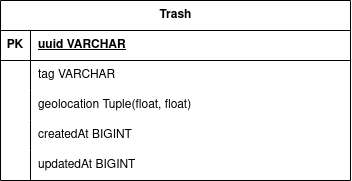
\includegraphics[width=12cm, height={\imgth}, keepaspectratio]{static/diagrams/trash-erd.png}
    \\
    \raggedright\small{Źródło: Opracowanie własne}
\end{figure}

\subsection{Diagramy sekwencji}

\forceindent Diagramy sekwencji przedstawiają istniejące w aplikacji serwerowej procesy, ścieżki oraz kolejność wykonywania operacji.

\begin{figure}[htbp]
    \textbf{\caption{Diagram logowania użytkownika}}
    \centering{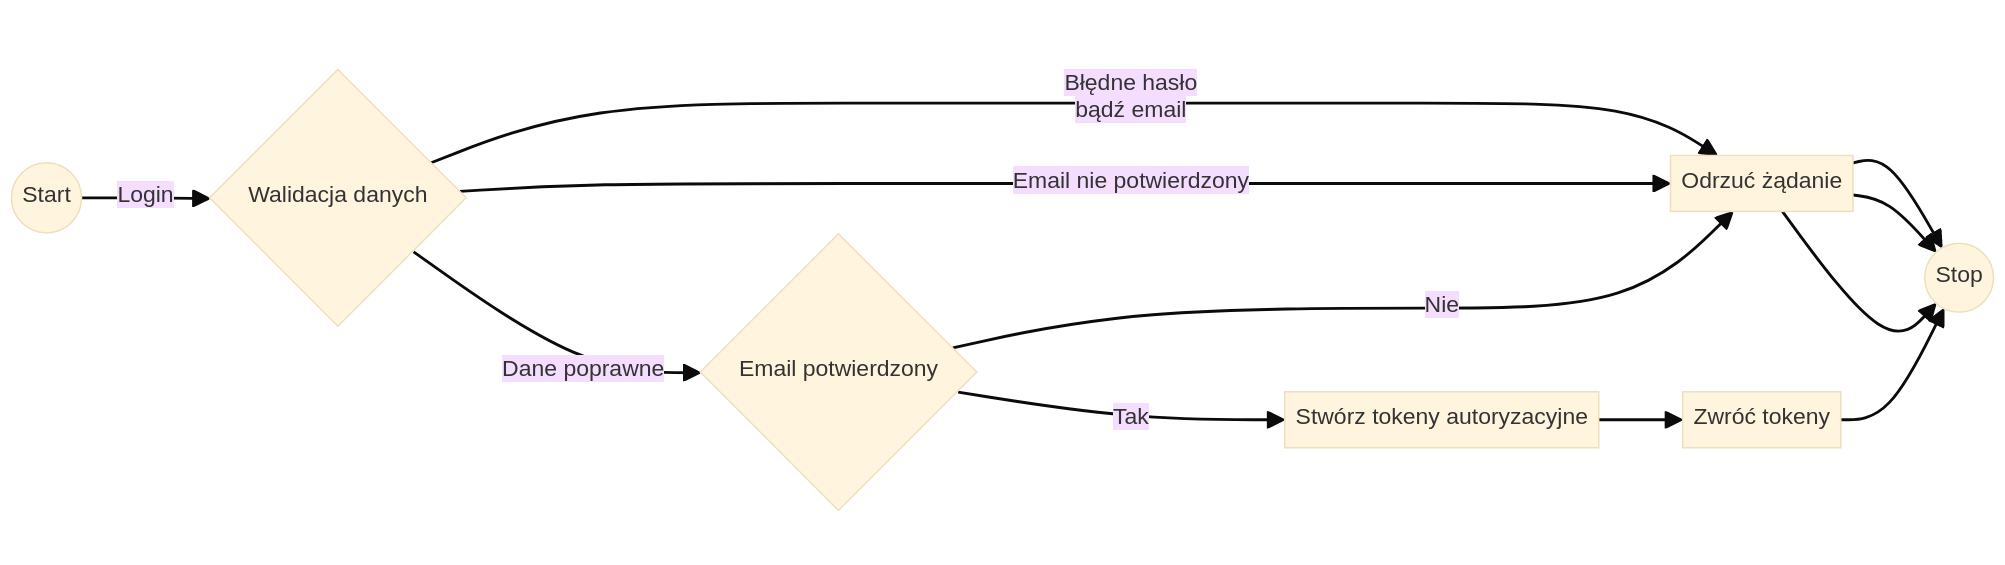
\includegraphics[width=15cm, height={\imgth}, keepaspectratio]{./static/diagrams/diagram-logowania.png}}\\
    \raggedright\small{Źródło: Opracowanie własne}
\end{figure}

Rysunek 3.3 przedstawia diagram procesu logowania użykownika wraz z drzewami decyzyjnymi.
Można owy proces podzielić na następujące odnogi:
\begin{itemize}[label=--]
    \item podanie błędnego hasła bądź adresu email -- odrzucenie żądania;
    \item brak potwierdzonego adresu email -- odrzucenie żądania;
    \item poprawne dane -- zwrócenie tokenów autoryzacyjnych.
\end{itemize}

\begin{figure}[htbp]
    \textbf{\caption{Diagram zmiany adresu email}}
    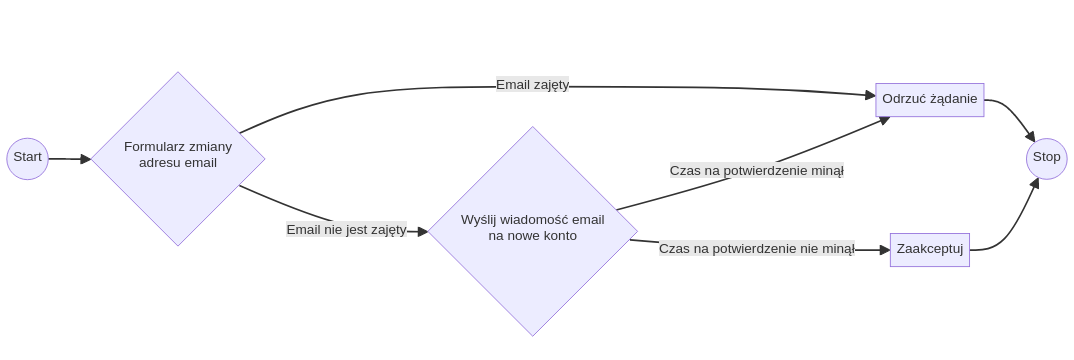
\includegraphics[width=15cm,height={\imgth}, keepaspectratio]{./static/diagrams/diagram-zmiany-adresu-email.png}\\
    \small{Źródło: Opracowanie własne}
\end{figure}

Rysunek 3.4 przedstawia diagram zmiany adresu email.
W ramach tego procesu wysyłana jest wiadomość na wskazany adres, w której to zawarty jest link do zmiany hasła.
Tenże link zawiera w sobie token o żywotności rzędu 24 godzin.
Odnogi decyzyjne w tym procesie można podzielić na następujące:
\begin{itemize}[label=--]
    \item adres email jest już zajęty -- odrzucenie żądania;
    \item token wygasł -- odrzucenie żądania;
    \item po kliknięciu na link adres email jest zmieniany.
\end{itemize}

\begin{figure}[htbp]
    \textbf{\caption{Diagram pobierania danych śmietników}}
    \vspace{0.55em}
    \centering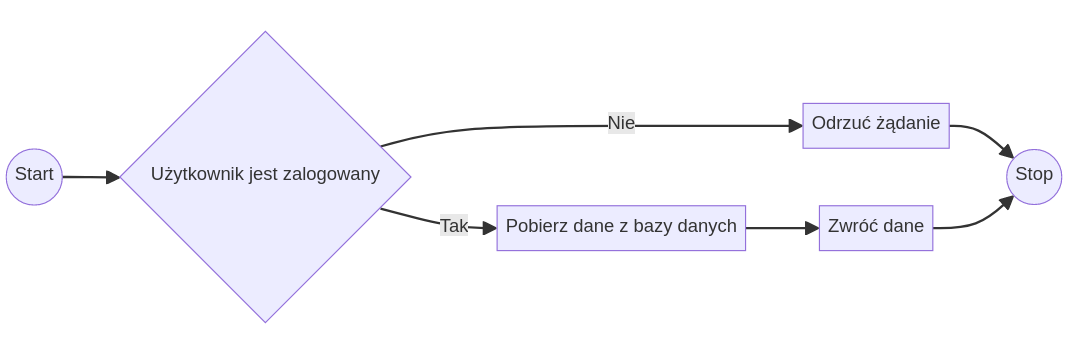
\includegraphics[width=15cm,height={\imgth}, keepaspectratio]{./static/diagrams/diagram-pobierania-danych-smietniczkow.png}\\
    \raggedright\small{Źródło: Opracowanie własne}
\end{figure}

Rysunek 3.5 przedstawia diagram pobierania danych śmietników.
Jego proces posiada jedno drzewko decyzyjne, którego wymogiem jest uwierzytelniony użytkownik.

\begin{figure}[htbp]
    \textbf{\caption{Diagram rejestracji użytkownika}}
    \vspace{0.55em}
    \centering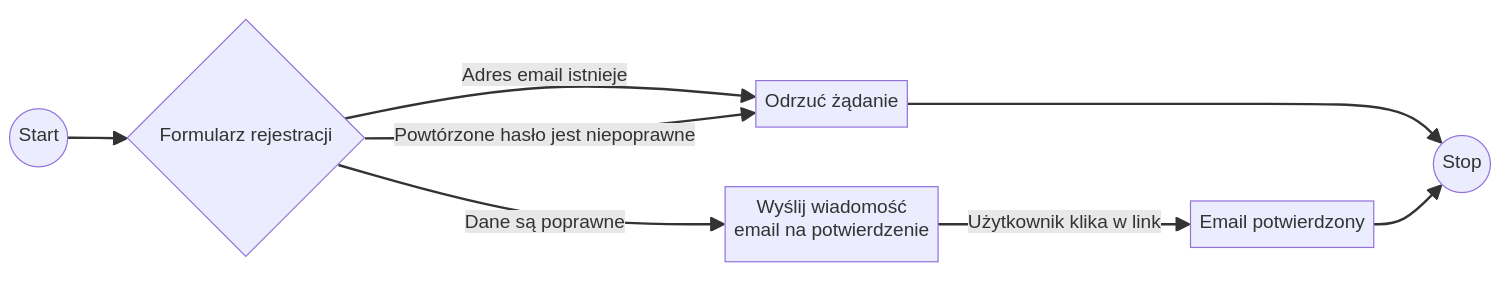
\includegraphics[width=15cm,height={\imgth}, keepaspectratio]{./static/diagrams/naprawiony-diagram-rejestracji.png}\\
    \raggedright\small{Źródło: Opracowanie własne}
\end{figure}

Rysunek 3.6 przedstawia diagram rejestracji użytkownika. Po wypełnieniu formularzu rejestracji użytkownik otrzymuje wiadomość email pod wskazanym adresem wraz z linkiem do potwierdzenia rejestracji. Po wejściu na witrynę, do której prowadzi link, konto użytkownika zostaje potwierdzone i może rozpocząć on korzystanie z aplikacji.

% \begin{figure}[h]
%     \textbf{\caption{Diagram resetu hasła użytkownika}}
%     \vspace{0.55em}
%     \centering\includegraphics[width=12cm,height={\imgth}, keepaspectratio]{./static/diagrams/diagram-resetu-hasła.png}\\
%     \raggedright\small{Źródło: Opracowanie własne}
% \end{figure}

\subsection{Diagram komunikacji między aplikacją serwerową i mobilną}

\forceindent Na rysunku 3.7 znajduje się diagram komunikacji między aplikacją serwerową i mobilną.
Diagram ten ma strukturę przedstawiającą interakcje między różnymi komponentami w systemie w kolejności ich występowania.

Na najwyższym poziomie diagram ilustruje interakcje między użytkownikiem (Użytkownik), aplikacją mobilną (Aplikacja Mobilna) i różnymi usługami zaplecza, w tym bramą API (Bramka API), usługą konta użytkownika (Serwis Konta Użytkownika), usługą zarządzania koszami na śmieci (Serwis Pojemników na Śmieci), repozytorium kont użytkowników (Repozytorium Konta Użytkownika), repozytorium koszy na śmieci (Repozytorium Pojemników na Śmieci) oraz usługą przesyłania wiadomości e-mail (Serwis Wiadomości Email).

Dodatkowo, diagram pokazuje mikrousługę wiadomości e-mail (Mikroserwis Wiadomości Email), która może być wywoływana w celu wysyłania powiadomień lub potwierdzeń do użytkownika. W trakcie całego procesu różne operacje zwracają wyniki (wynik operacji), które są przekazywane z powrotem przez system, ostatecznie dostarczając użytkownikowi widok lub odpowiedź za pośrednictwem aplikacji mobilnej.

Sekwencja interakcji jest asynchroniczna i opiera się na modelu żądanie-odpowiedź, w którym działania użytkownika wyzwalają serię żądań, które przepływają przez system i skutkują serią odpowiedzi.

\begin{sidewaysfigure}
    \textbf{\caption{Diagram komunikacji}}
    \vspace{3.5em}
    \centering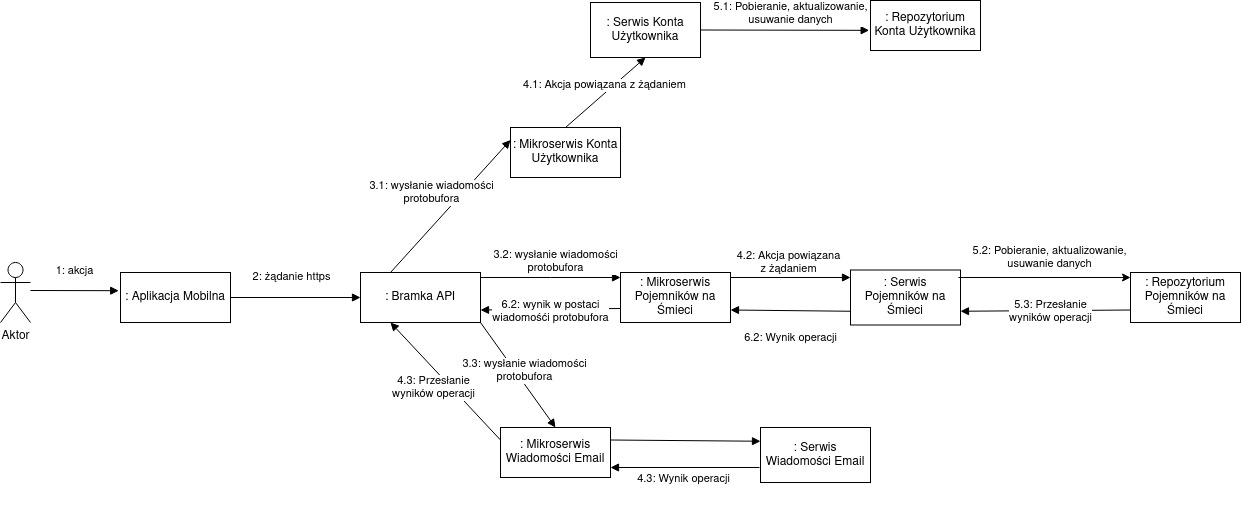
\includegraphics[width=\fittingimage, keepaspectratio]{static/diagrams/diagram-komunikacji.jpg}
    \\
    \raggedright\small{Źródło: opracowanie własne}
\end{sidewaysfigure}

\subsection{Testy automatyczne aplikacji serwerowej}
\forceindent Aplikacja serwerowa została przetestowana za pomocą testów jednostkowych, integracyjnych oraz testów obciążaniowych.

W przypadku testów jednostkowych, nie pobrano pomiarów związanych z pokryciem kodu źródłowego, z uwagi na małą ich miarodajność. Aplikacja została w przeważającej mierze przetestowana za pomocą testów integracyjnych, z uwagi na małą ilość ścieżek decyzjnych w kodzie.

Mikroserwis pojemników na śmieci posiada łącznie 6 testów jednostkowych, co przedstawione jest na rysunku 3.8, oraz 9 testów integracyjnych (rysunek 3.9). Przekłada się to na wysoką odporność na potencjalne błędy.

\begin{figure}[htbp]
    \textbf{\caption{Wyniki testów jednostkowych mikroserwisu pojemników na śmieci}}
    \vspace{0.55em}
    \centering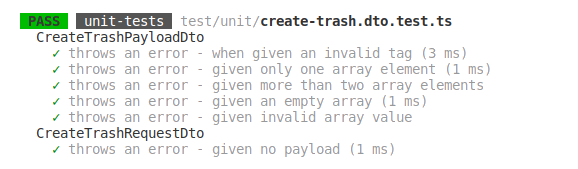
\includegraphics[width=12.5cm,height={\imgth}, keepaspectratio]{./static/trash-unit.png}
    \\
    \raggedright \small{Źródło: Opracowanie własne}
\end{figure}

\begin{figure}[htbp]
    \textbf{\caption{Wyniki testów integracyjnych mikroserwisu pojemników na śmieci}}
    \vspace{0.55em}
    \centering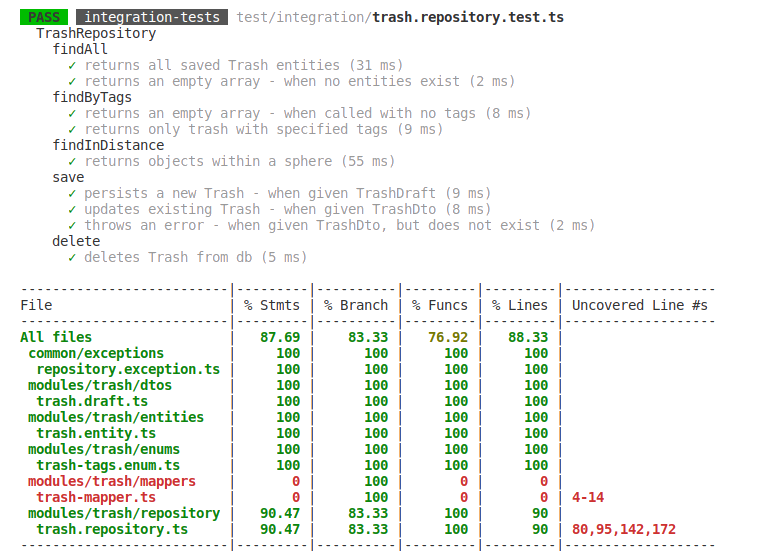
\includegraphics[width=12.5cm,height={\imgth}, keepaspectratio]{./static/trash-integration-tests.png}
    \\
    \raggedright \small{Źródło: Opracowanie własne}
\end{figure}

Mikroserwis kont użytkownika posiada łącznie 8 testów jednostkowych oraz 43 testy integracyjne.
Przetestowane zostały ścieżki związane z logowaniem, rejestracją oraz zmianami w danych konta użytkowika.

\begin{figure}[htbp]
    \textbf{\caption{Wyniki testów jednostkowych mikroserwisu konta użytkownika}}
    \vspace{0.55em}
    \centering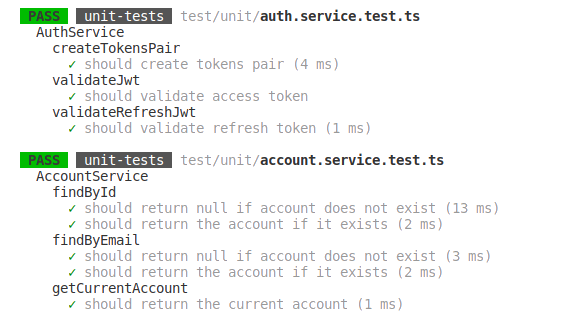
\includegraphics[width=12.5cm,height={\imgth}, keepaspectratio]{./static/accounts-unit.png}
    \\
    \raggedright \small{Źródło: Opracowanie własne}
\end{figure}

\begin{figure}[htbp]
    \textbf{\caption{Wyniki testów integracyjnych mikroserwisu kont użytkownika}}
    \vspace{0.55em}
    \centering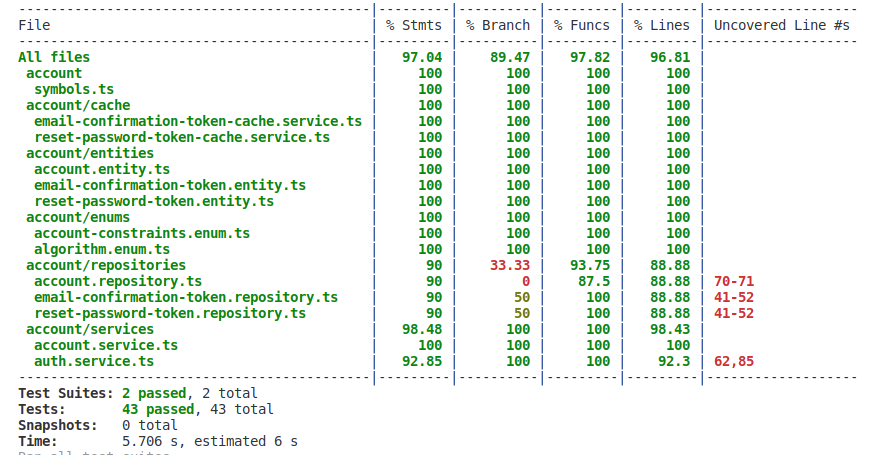
\includegraphics[width=12.5cm,height={\imgth}, keepaspectratio]{./static/accounts-integration-tests.png}
    \\
    \raggedright \small{Źródło: Opracowanie własne}
\end{figure}

\newpage

\subsection{Aplikacja mobilna}

\forceindent Implementując naszą aplikację mobilną w języku Swift, wybraliśmy ten język ze względu na jego wydajność i elastyczność. Jednak podczas procesu tworzenia napotkaliśmy wiele wyzwań, które były spowodowane zarówno architekturą aplikacji, jak i wbudowanymi rozwiązaniami dostępnymi w języku Swift. Podobnie jak w przypadku frameworka NestJS w naszej aplikacji serwerowej, Swift dostarcza wiele gotowych rozwiązań i narzędzi, ale często są one mało intuicyjne lub mogą zawierać błędy. Nasz zespół musiał się zmierzyć z tymi problemami i dostosować te rozwiązania do naszych potrzeb. Jednocześnie stworzyliśmy własne komponenty i moduły, które integrowaliśmy z istniejącym kodem, aby zapewnić płynność działania i najlepsze wrażenia z użytkowania naszej aplikacji.

Aplikację można podzielić na cztery moduły, które obejmują:

\begin{itemize}
    \item Moduł Autoryzacji:
          \begin{itemize}
              \item Użytkownik ma możliwość zalogowania się do aplikacji, podając swój adres e-mail i hasło.
              \item Tworzenie konta polega na dostarczeniu danych użytkownika oraz potwierdzeniu konta poprzez link wysłany na podany adres e-mail.
              \item Istnieje również opcja odzyskiwania zapomnianego hasła, gdzie użytkownik może podać swój adres e-mail i przejść przez proces resetowania hasła za pośrednictwem linku wysłanego na jego e-mail.
          \end{itemize}
\end{itemize}

\begin{itemize}
    \item Moduł Dodawania Śmietników:
          \begin{itemize}
              \item Aby dodać nowy śmietnik, użytkownik przechodzi do dedykowanego panelu dostępnego na stronie głównej.
              \item Po dodaniu zdjęcia, model uczenia maszynowego rozpoznaje rodzaj śmietnika na zdjęciu.
              \item Użytkownik ma możliwość edytowania tej informacji oraz podania dokładnego adresu.
              \item Po wprowadzeniu danych, punkt zostaje zaznaczony na mapie.
          \end{itemize}
\end{itemize}

\begin{itemize}
    \item Strona Główna:
          \begin{itemize}
              \item Na stronie głównej znajduje się mapa, na której widoczne są oznaczone śmietniki.
              \item Mapę można przeszukiwać za pomocą wbudowanej wyszukiwarki znajdującej się w górnej części aplikacji.
              \item Po kliknięciu na oznaczenie, użytkownik otrzymuje informacje dotyczące wybranego śmietnika.
          \end{itemize}
\end{itemize}

\begin{itemize}
    \item Panel Użytkownika:
          \begin{itemize}
              \item W panelu użytkownika użytkownik może zarządzać swoimi danymi, które można edytować.
              \item Istnieje przycisk przekierowujący użytkownika do ustawień aplikacji.
              \item Użytkownik ma możliwość zmiany motywu aplikacji na jasny lub ciemny.
              \item Dostępna jest opcja pełnego wylogowania z aplikacji.
          \end{itemize}
\end{itemize}

\subsection{Stylowanie iterfejsu użytkownika}
\forceindent{Stylowanie interfejsu użytkownika było istotnym aspektem projektu. Dzięki SwiftUI, możliwe było zdefiniowanie wyglądu i stylu poszczególnych widoków w sposób deklaratywny. Przykładowo, używając atrybutów takich jak .font(), .foregroundColor() czy .background(), można było łatwo dostosować czcionki, kolory i tła elementów interfejsu użytkownika.}

Dodatkowo, aplikacja wykorzystuje dostępne narzędzia do tworzenia spersonalizowanych widoków oraz dostosowywania przycisków i ikon. Stylowanie było przemyślane tak, aby spełnić oczekiwania użytkowników i zachować spójność z wytycznymi projektu.

\subsection{Widoki aplikacji mobilnej}

\forceindent{Na rysunku 3.12 widoczny jest ekran startowy aplikacji mobilnej. Umożliwia on przejście do procesu rejestracji poprzez przycisk „Dołącz teraz” (ang. \textit{Join Now}) oraz do ekranu logowania przez kliknięcie w przycisk „Zaloguj się” (ang. \textit{Login}). }

\begin{figure}[htb]
    \textbf{\caption{Ekran startowy aplikacji mobilnej}}
    \vspace{0.55em}
    \centering
    
\includegraphics[width=9cm, height=14cm, keepaspectratio]{./static/mobile/start-page.jpg}\\
    \raggedright\small{Źródło: Opracowanie własne}
\end{figure}

\newpage
\forceindent{Rysunek 3.13 przedstawia widok rejestracji, dzięki któremu użytkownik może założyć konto, podając nazwę użytkownika, adres e-mail oraz hasło. W celu dodatkowej walidacji, hasło należy wprowadzić dwa razy. Po prawidłowym wpisaniu danych, należy kliknąć przycisk „Zarejestruj się” (ang. \textit{Register}). Z ekranu rejestracji istnieje możliwość łatwego przejścia do ekranu logowania poprzez kliknięcie w napis „Zaloguj się” (ang. \textit{Login}).}

\begin{figure}[htb]
    \textbf{\caption{Widok rejestracji}}
    \vspace{0.55em}
    \centering
    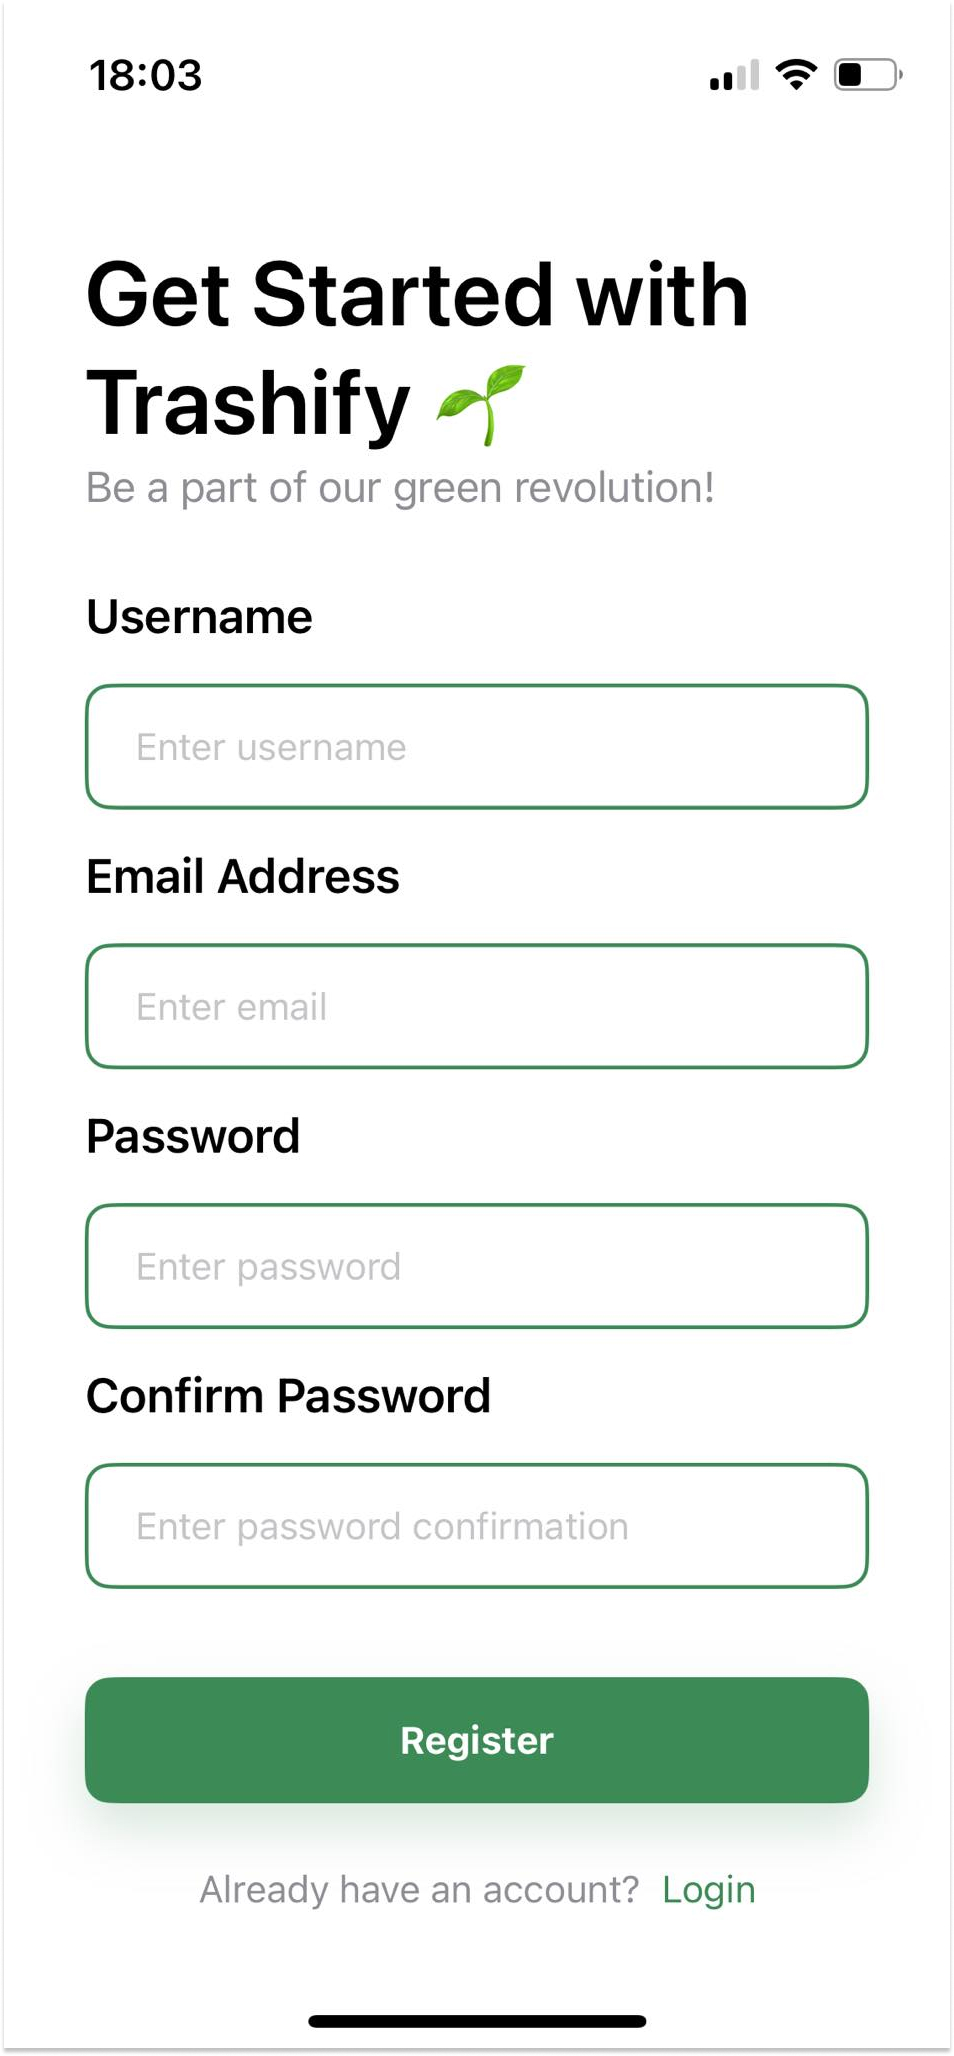
\includegraphics[width=9cm, height=14cm, keepaspectratio]{./static/mobile/register.jpg}\\
    \raggedright\small{Źródło: Opracowanie własne}
\end{figure}

\newpage
\forceindent{Aby zalogować się do aplikacji, użytkownik musi podać swój adres email oraz hasło, co widoczne jest na rysunku 3.14. Proces logowania zatwierdza się, klikając przycisk „Zaloguj się” (ang. \textit{Login}). Z ekranu logowania istnieje również możliwość przejścia do panelu odzyskiwania hasła poprzez kliknięcie w napis „Zapomniałeś hasła?” (ang. \textit{Forgot password?}) oraz do ekranu rejestracji przez kliknięcie w „Zarejestruj się” (ang. \textit{Register}).}

\begin{figure}[htb]
    \textbf{\caption{Ekran logowania}}
    \vspace{0.55em}
    \centering
    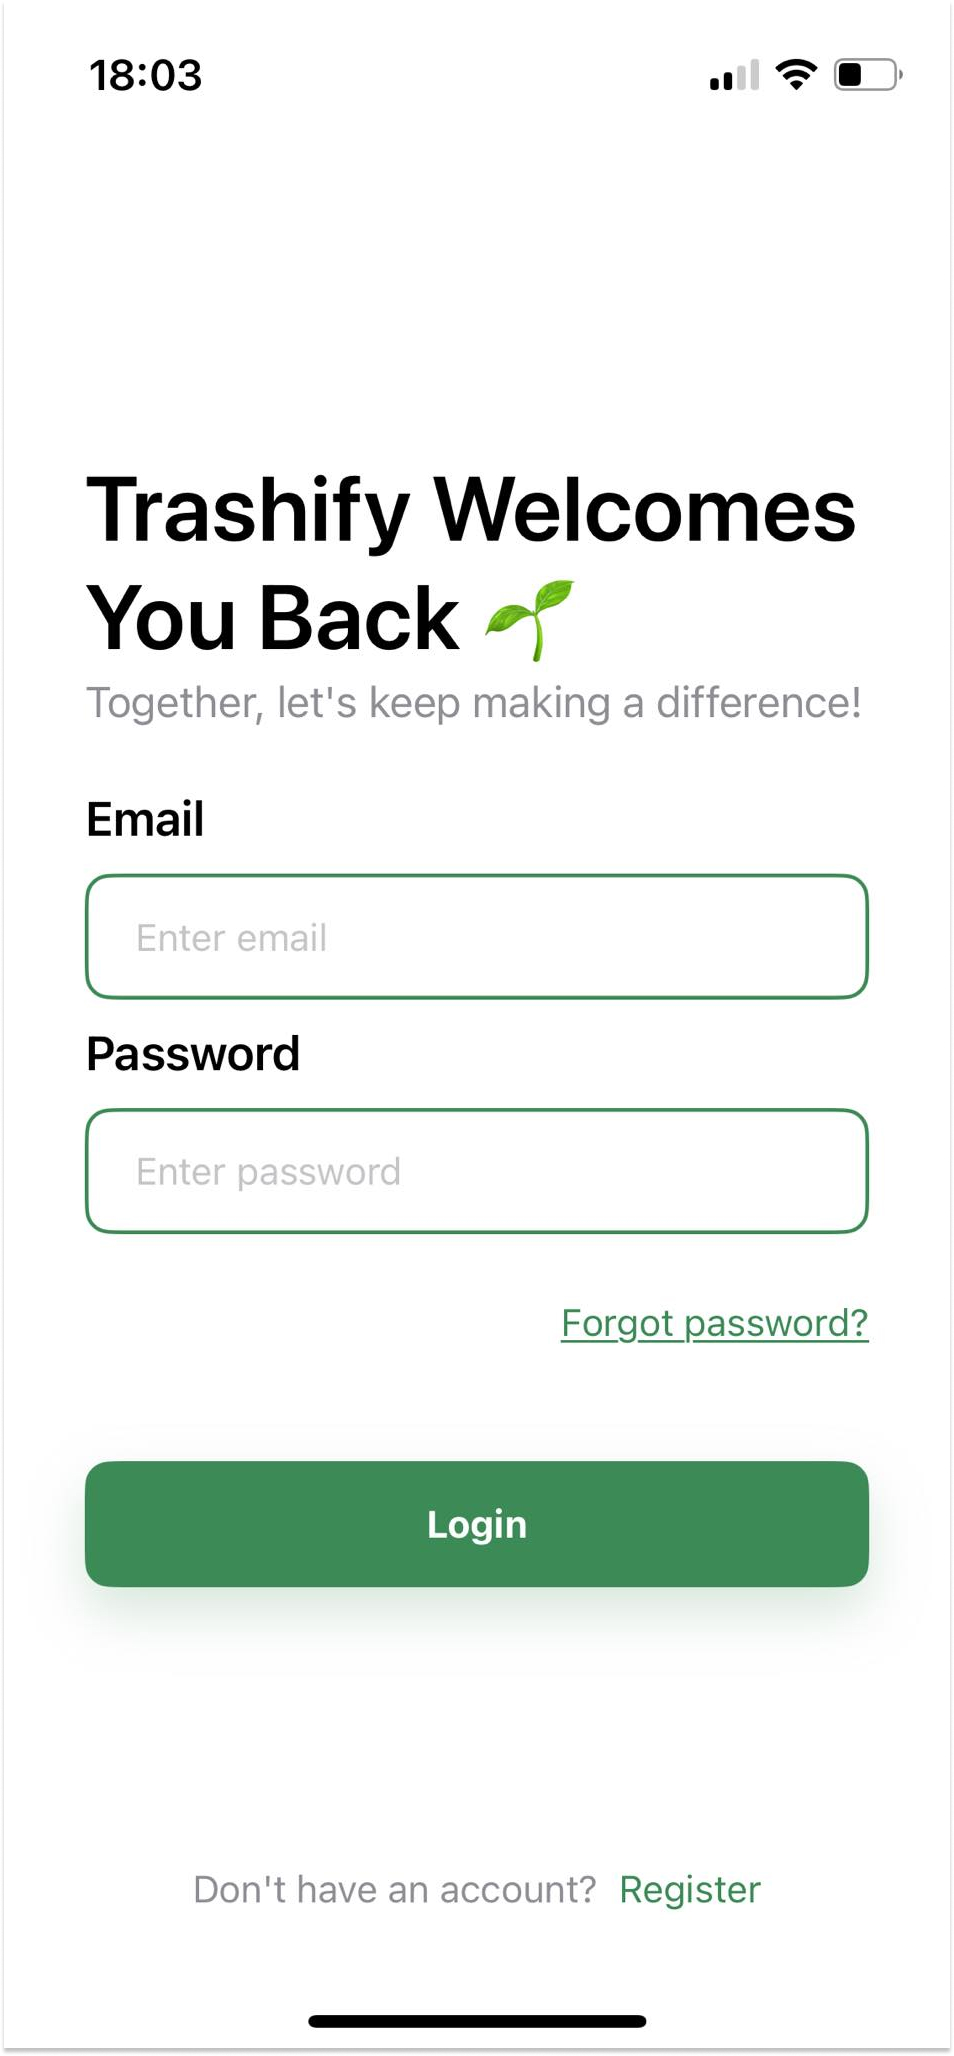
\includegraphics[width=9cm, height=14cm, keepaspectratio]{./static/mobile/login.jpg}\\
    \raggedright\small{Źródło: Opracowanie własne}
\end{figure}

\newpage
\forceindent{Rysunek 3.15 przedstawia panel odzyskiwania hasła, który to wykorzystywany jest przez użytkowników w celu odzyskania hasła. Użytkownik powinien podać adres email powiązany z kontem, a następnie zatwierdzić operację za pomocą przycisku „Resetuj Hasło” (ang. \textit{Reset Password}). Po prawidłowym wykonaniu tej operacji, na podany adres email zostanie wysłana wiadomość z linkiem umożliwiającym odzyskanie hasła.}

\begin{figure}[htb]
    \textbf{\caption{Panel odzyskiwania hasła}}
    \vspace{0.55em}
    \centering
    
\includegraphics[width=9cm, height=14cm, keepaspectratio]{./static/mobile/forgot-password.jpg}\\
    \raggedright\small{Źródło: Opracowanie własne}
\end{figure}

\newpage
\forceindent{Strona główna (rysunek 3.16) prezentuje mapę z oznaczonymi lokalizacjami śmietników. Każdy typ śmietnika jest reprezentowany przez unikalny kolor i ikonę. Kliknięcie na tag śmietnika wyświetla dodatkowe informacje o danym punkcie. Na górze strony znajduje się pole tekstowe umożliwiające wyszukiwanie określonych lokalizacji. Po wpisaniu początku nazwy miasta, automatycznie pojawia się lista sugerowanych pasujących miejsc. Użytkownik może wybrać interesującą go lokalizację z tej listy. Na dole strony umieszczono menu nawigacyjne, dzięki któremu można łatwo poruszać się po aplikacji.}

\begin{figure}[htb]
    \textbf{\caption{Strona główna}}
    \vspace{0.55em}
    \centering
    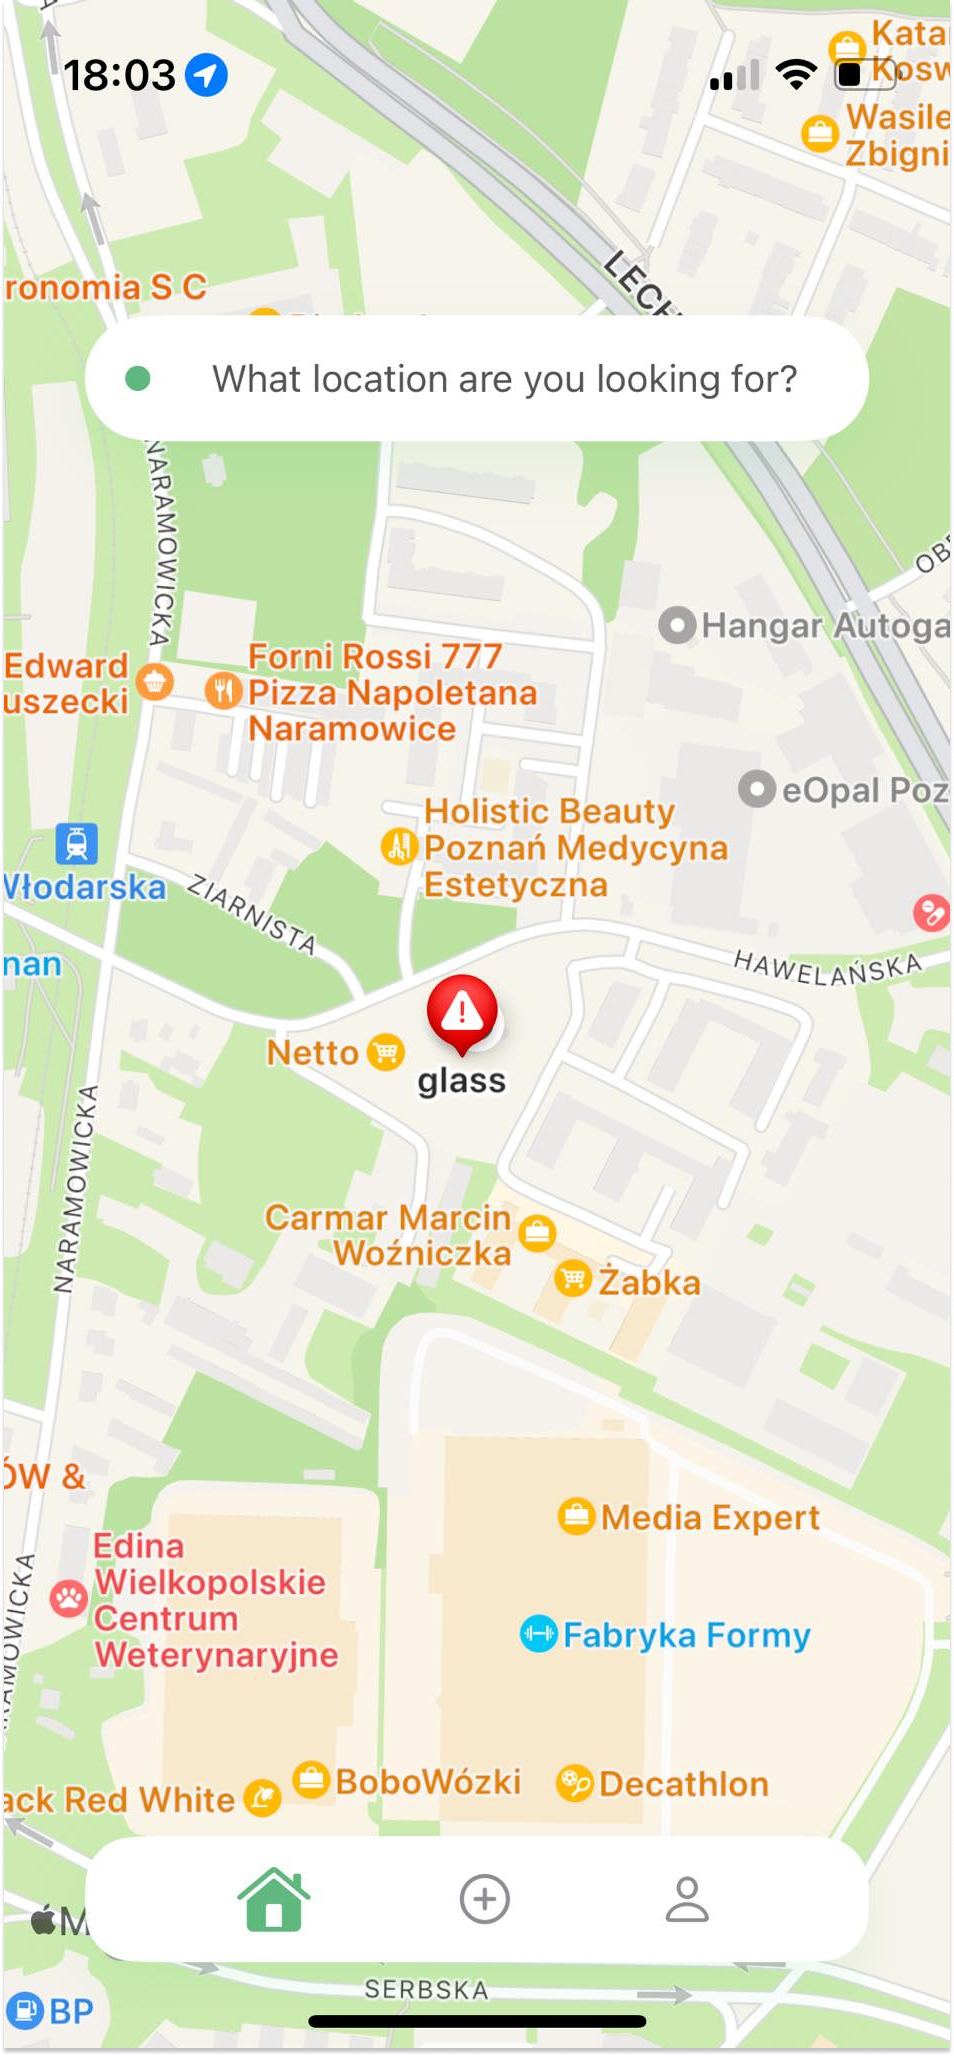
\includegraphics[width=9cm, height=14cm, keepaspectratio]{./static/mobile/home-page.jpg}\\
    \raggedright\small{Źródło: Opracowanie własne}
\end{figure}

\newpage
\forceindent{Rysunek 3.17 przedstawia panel dodawnia punktów na mapie. Celem dodania nowego punktu na mapie, użytkownik powinien wybrać ikonę plusa w menu. Po otwarciu panelu, pierwszym krokiem jest dodanie zdjęcia. Zastosowany model uczenia maszynowego automatycznie rozpozna typ śmietnika. Jeśli rozpoznanie jest błędne, użytkownik ma możliwość ręcznej zmiany typu. Następnie, po weryfikacji typu śmietnika i lokalizacji, operację dodania punktu zatwierdza się przyciskiem „Zapisz” (ang. \textit{Save}).}

\begin{figure}[htb]
    \textbf{\caption{Panel dodawania punktów}}
    \vspace{0.55em}
    \centering
    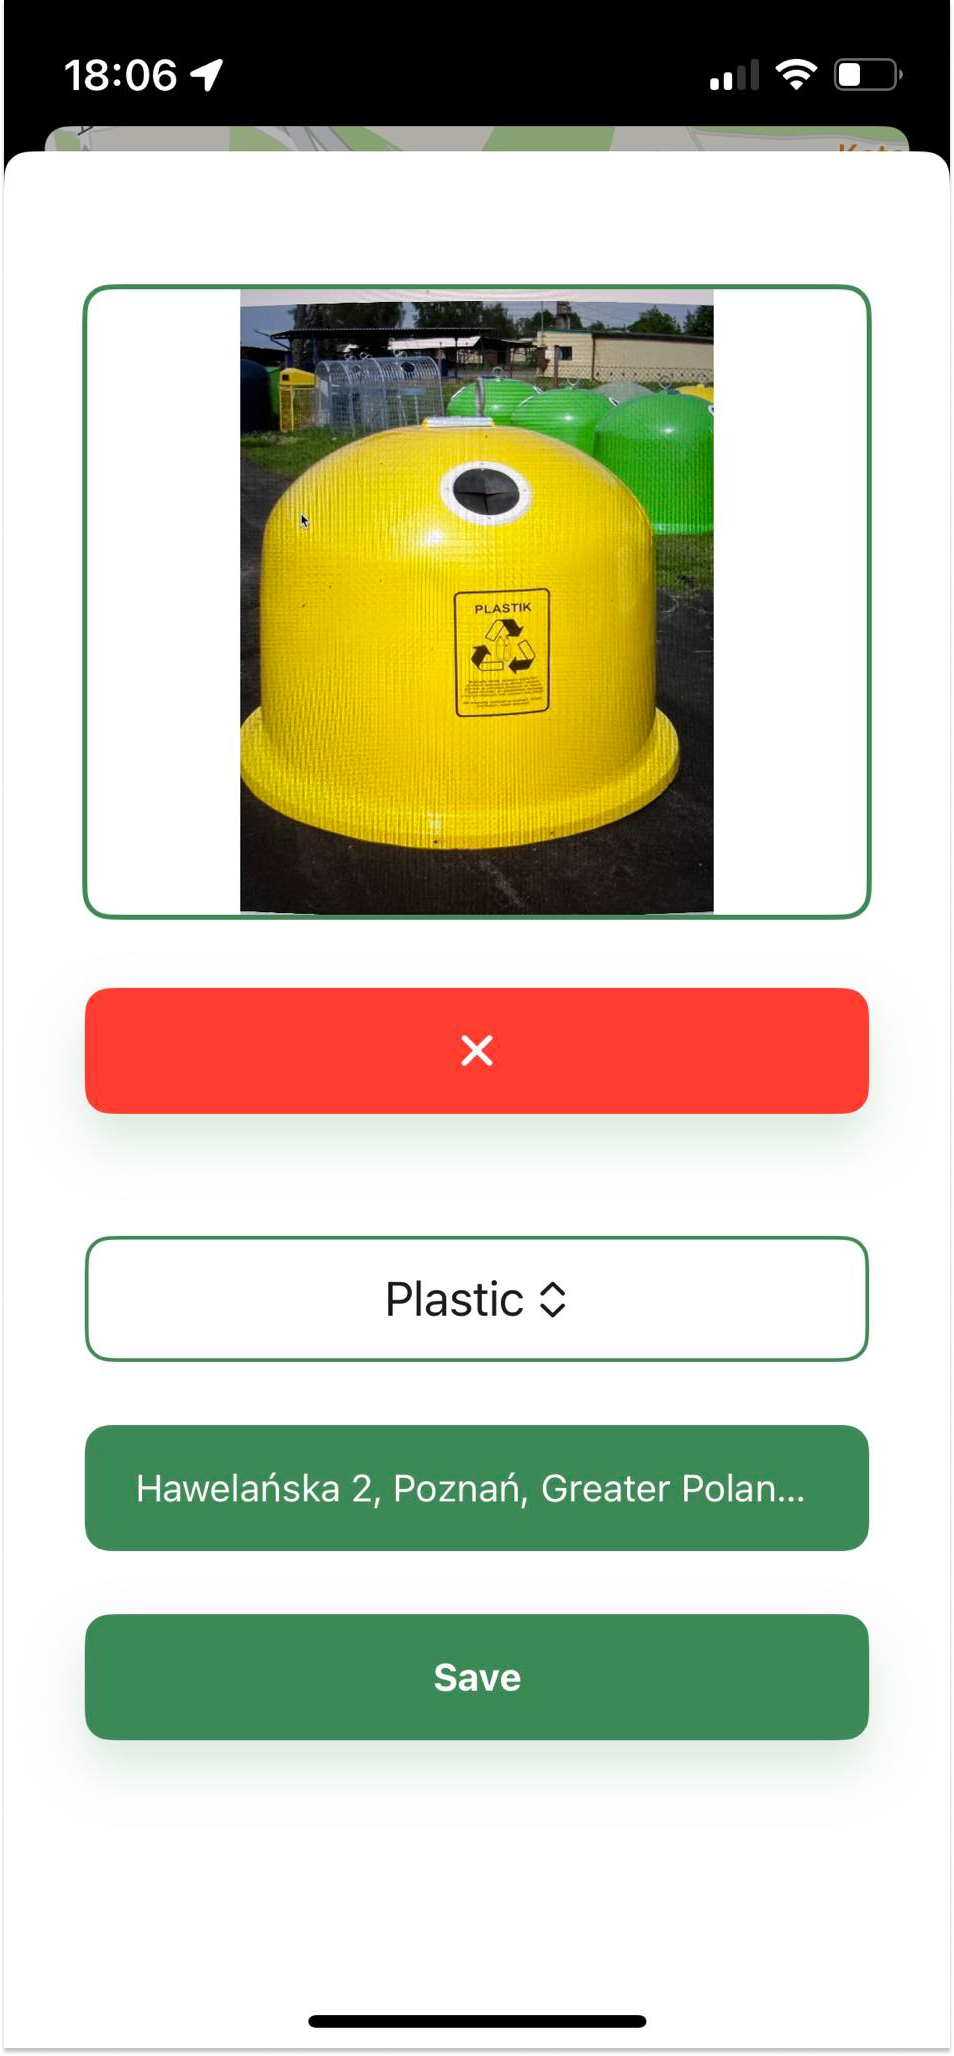
\includegraphics[width=8cm, height=14cm, keepaspectratio]{./static/mobile/add-trash.jpg}\\
    \raggedright\small{Źródło: Opracowanie własne}
\end{figure}

\newpage
\forceindent{Panel użytkownika (rysunek 3.18) umożliwia edycję nazwy użytkownika oraz adresu email. Proces edycji rozpoczyna się od kliknięcia w przycisk „Edytuj” (ang. \textit{Edit}), co przekierowuje do odpowiedniego panelu edycyjnego. Funkcja „Ustawienia dostępu” (ang. \textit{Access settings}) pozwala na przeniesienie do sekcji ustawień, gdzie użytkownik może konfigurować uprawnienia aplikacji. Za pomocą suwaka trybu ciemnego (ang. \textit{dark mode}) istnieje możliwość zmiany wyglądu aplikacji z jasnego na ciemny i odwrotnie. Opcja „Wyloguj się” (ang. \textit{Sign out}) umożliwia bezpieczne wylogowanie się z konta.}

\begin{figure}[htb]
    \textbf{\caption{Panel użytkownika}}
    \vspace{0.55em}
    \centering
    \includegraphics[width=8cm, height=14cm, keepaspectratio]{./static/mobile/panel-użytkownika.png}\\
    \raggedright\small{Źródło: Opracowanie własne}
\end{figure}

\newpage
\forceindent{Panele edycji nazwy użytkownika i adresu email widoczne są odpowiednio na rysunkach 3.19 oraz 3.20. Celem edycji nazwy użytkownika, należy wpisać nową nazwę, a następnie zatwierdzić zmianę, klikając przycisk „Zapisz” (ang. \textit{Save}). Proces zmiany adresu email przebiega w identyczny sposób: użytkownik wpisuje nowy adres email i zatwierdza zmianę za pomocą tego samego przycisku „Zapisz” (ang. \textit{Save}).}

\begin{figure}[htbp]
    \textbf{\caption{Widok aktualizowania adresu email}}
    \centering
    \vspace{0.55em}
    
\includegraphics[width=8cm, height=9cm, keepaspectratio]{./static/mobile/update-email.jpg}\\
    \raggedright\small{Źródło: Opracowanie własne}
\end{figure}
\begin{figure}[htbp]
    \textbf{\caption{Widok aktualizowania hasła użytkownika}}
    \centering
    \vspace{0.55em}
    
\includegraphics[width=8cm, height=9cm, keepaspectratio]{./static/mobile/update-password.jpg}\\
    \raggedright\small{Źródło: Opracowanie własne}
\end{figure}

\subsection{Problemy z realizacją aplikacji mobilnej}
\forceindent{W trakcie pracy nad projektem aplikacji mobilnej, który był realizowany w grupie, napotkaliśmy kilka istotnych problemów. Pierwszym z nich był problem z wyświetlaniem punktów na mapie, gdzie główną trudnością było skomunikowanie aplikacji z danymi geolokacyjnymi, które były aktualizowane w czasie rzeczywistym w modelu. To spowodowało wyzwania związane z odpowiednim pobieraniem i wyświetlaniem tych danych na interfejsie użytkownika. Kolejnym problemem była efektywność wyszukiwania punktów na mapie, które miało być dynamiczne i responsywne. Jednak napotkaliśmy trudności związane z aktualizacją koordynatów punktów w modelu oraz ich odwzorowaniem na mapie. To wymagało starannej synchronizacji między danymi w modelu a ich reprezentacją na mapie.}

Całość komunikacji pomiędzy bramką interfejsu aplikacji a mikroserwisami, oparta jest na protokole gRPC. Wiadomości wysyłane są za pomocą protobuforów, a komunikacja z klientem oparta jest na protokole HTTPS.

W trakcie pracy z aplikacją serwerową, zespół napotkał problemy związane z komunikacją gRPC oraz paczką class-validator, która to powodowała ciche przerwanie operacji, bez żadnej informacji o błędzie.
\subsection{Algorytmy i techniki wykorzystane do nauki modelu uczenia maszynowego}

\subsubsection{Konwolucyjne sieci neuronowe}
\forceindent W projekcie Trashify wykorzystano wstępnie wytrenowaną konwolucyjną sieć neuronową (ang. \textit{Convolutional neural network -- CNN}) z ekstraktorem funkcji ,,Image Feature Print V2`` w CreateML, usprawniając proces analizy danych obrazu dla roważanego zbioru danych.

,,Image Feature Print V2`` jest narzędziem w CreateML, które znacznie usprawnia proces ekstrakcji cech. Wykorzystując je wraz ze wstępnie wytrenowaną CNN, skutecznie dostosowano sieć do unikalnych cech roważanego zbioru danych. Ta kombinacja pozwoliła na zniuansowaną analizę cech przestrzennych, kluczową dla identyfikacji określonych wzorców na rozpatrywanych obrazach, takich jak rozróżnianie kolorów, oznaczeń, kształtów pojemników.

Zastosowana metoda polegała na dostrojeniu wstępnie wytrenowanego modelu do analizowanego zbioru danych, co jest procesem zarówno efektywnym czasowo, jak i skutecznym. To dostrojenie było niezbędne do dostosowania możliwości modelu do konkretnych celów projektowych w zakresie rozpoznawania i klasyfikacji obrazów.

\subsubsection{Uczenie nadzorowane}
\forceindent W ramach pracy zastosowano uczenie nadzorowane, opierając się na oznaczonym zbiorze danych. Każdy obraz w tym zbiorze danych został precyzyjnie oznaczony etykietą identyfikującą konkretny typ kontenera. W trakcie treningu wykorzystywana konwolucyjna sieć neuronowa przeszła proces nauki, podczas którego zapoznawała się z charakterystycznymi cechami i wzorcami obrazów, a następnie łączyła je z odpowiadającymi etykietami. Ten proces umożliwił modelowi skuteczne przyswajanie cech definiujących każdy rodzaj kontenera.

W celu oceny wydajności rozważanego modelu korzystano z różnych miar, takich jak dokładność, precyzja, przywołanie, czułość i miara F1. Te wskaźniki dostarczały istotnych informacji na temat zdolności modelu do poprawnego identyfikowania poszczególnych typów kontenerów. Praktyczne zastosowanie tych miar pozwoliło na szczegółową analizę skuteczność rozpatrywanego modelu w analizowanego zadania, co było kluczowe dla oceny jego przydatności i precyzji w identyfikacji różnorodnych kontenerów.

\subsection{Proces szkolenia}
\forceindent Proces szkoleniowy obejmował dostarczanie dużej liczby oznaczonych obrazów do sieci CNN. Sieć przetworzyła te obrazy przez swoje warstwy, dostosowując swoje wewnętrzne parametry (wagi i odchylenia) na podstawie błędu pomiędzy prognozami a rzeczywistymi etykietami (propagacja wsteczna).
Ten iteracyjny proces trwał, dopóki model nie osiągnął zadowalającego poziomu dokładności, wskazującego na jego zdolność do dokładnej klasyfikacji nowych, niewidzianych obrazów.

\subsection{Wyzwania i rozważania}
\forceindent Kluczowym wyzwaniem w szkoleniu CNN do zadań klasyfikacji obrazów, jest zapewnienie wystarczająco dużego i zróżnicowanego zbioru danych, aby zapobiec nadmiernemu dopasowaniu i poprawić zdolność modelu do uogólniania.
Dodatkowo, kluczowe znaczenie ma zrównoważenie zbioru danych w celu uniknięcia nierównowagi klas, która mogłaby skłaniać model w kierunku częściej występujących klas. Zespół projektowy zwrócił na to szczególną uwagę, aby zapewnić, że model będzie w stanie rozpoznawać wszystkie typy kontenerów z wysoką dokładnością.

\subsection{Analiza wydajności modelu klasyfikacji pojemników}

\forceindent Analiza wydajności modelu klasyfikacji pojemników na odpady przeprowadzona została poprzez ocenę trzech kluczowych wskaźników: precyzji, czułości oraz miary F1 dla różnych kategorii pojemników na odpady. W celu ułatwienia interpretacji wyników, wyniki te zostały odniesione do tabeli referencyjnej, która określa granice procentowe dla oceny skuteczności modelu.

\subsubsection{Punkt odniesienia: Tabela oceny wyników}
\forceindent Do oceny wyników modelu została wykorzystana tabela referencyjna 3.2, która definiuje granice procentowe dla różnych poziomów skuteczności modelu.

\begin{table}[ht]
    \small
    \centering
    \textbf{\caption{Tabela referencyjna do oceny wyników modelu klasyfikacji pojemników}}
    \vspace{0.55em}
    \begin{tabular}{|c|c|c|c|}
        \hline
        Ocena        & Precyzja (\%)      & Czułość (\%)       & Miara F1             \\ \hline
        Niska        & < 50               & < 50               & < 0.5                \\ \hline
        Umiarkowana  & 50 -- 69            & 50 -- 69            & 0.5 -- 0.69           \\ \hline
        Dobra        & 70 -- 84            & 70 -- 84            & 0.7 -- 0.84           \\ \hline
        Bardzo dobra & \textgreater{}= 85 & \textgreater{}= 85 & \textgreater{}= 0.85 \\ \hline
    \end{tabular}
    \label{tab:my-table}
    \\
    \vspace{0.55em}
    \raggedright\small{Źródło: Opracowanie własne}
\end{table}

\subsubsection{Pojemniki na plastik}
\begin{itemize}
    \item Uzyskana precyzja wyniosła 55\%, co klasyfikuje się jako umiarkowaną efektywność modelu w identyfikacji pojemników plastikowych.
    \item Czułość osiągnięta na poziomie 70\% świadczy o zdolności modelu do efektywnego wykrywania plastikowych pojemników.
    \item Miara F1, wynosząca 0,616, wskazuje na umiarkowaną równowagę między precyzją a czułością.
\end{itemize}

\subsubsection{Pojemniki na papier}
\begin{itemize}
    \item Precyzja na poziomie 74\% świadczy o wysokiej skuteczności modelu w identyfikacji pojemników papierowych.
    \item Czułość wynosząca 64\% wskazuje na dość dobre umiejętności modelu w wykrywaniu pojemników papierowych w zbiorze danych.
    \item Miara F1, osiągając 0,686, potwierdza dobrą równowagę między precyzją a czułością.
\end{itemize}

\subsubsection{Pojemniki na odpady mieszane}
\begin{itemize}
    \item Precyzja wynosząca 60\% wskazuje na umiarkowaną skuteczność modelu w tej kategorii.
    \item Czułość na poziomie 59\% również świadczy o umiarkowanej zdolności do wykrywania pojemników na odpady mieszane.
    \item Miara F1, wynosząca 0.595, odzwierciedla umiarkowaną równowagę między precyzją a czułością.
\end{itemize}

\subsubsection{Pojemniki na szkło}
\begin{itemize}
    \item Precyzja na poziomie 72\% wskazuje na dobrą skuteczność modelu w identyfikacji pojemników szklanych.
    \item Czułość wynosząca 55\% wskazuje na umiarkowane ryzyko przeoczenia obrazów pojemników szklanych.
    \item Miara F1 na poziomie 0,624 świadczy o umiarkowanej równowadze między precyzją a czułością.
\end{itemize}

\subsubsection{Pojemniki na odpady biodegradowalne}
\begin{itemize}
    \item Precyzja wynosząca 65\% świadczy o dość dobrej skuteczności modelu w tej kategorii.
    \item Czułość również na poziomie 65\% wskazuje na zdolność do efektywnego wykrywania pojemników biodegradowalnych.
    \item Miara F1 wynosząca 0,65 pokazuje dobrą równowagę między precyzją a czułością.
\end{itemize}


\subsection{Wymagania sprzętowe i oprogramowania dla aplikacji mobilnej}
\begin{itemize}[label=--]
    \item Komputer z systemem operacyjnym macOS Sonoma lub nowszym
    \item Oprogramowanie Xcode 15 lub nowsze, dostępne do pobrania z App Store
\end{itemize}

\subsection{Instalacja aplikacji mobilnej}

\subsubsection{Otwieranie projektu w Xcode }
\begin{itemize}[label=--]
    \item Otwórz Xcode.
    \item Wybierz File > Open i znajdź sklonowany katalog projektu.
    \item Wybierz plik .xcodeproj i kliknij Open
\end{itemize}

\subsubsection{Uruchomienie projektu aplikacji mobilnej}
\begin{itemize}
    \item Wybierz urządzenie docelowe w Xcode.
    \item Kliknij przycisk Run lub użyj skrótu Cmd + R, aby uruchomić aplikację.
\end{itemize}

\subsection{Instrukcja developerska aplikacji serwerowej}

\forceindent Celem uruchomienia lokalnej instancji aplikacji serwerowej, użytkownik potrzebuje następujących narzędzi:
\begin{itemize}[label=--]
    \item środowiska rozruchomieniowego Node.js w wersji 20.9 bądź nowszej;
    \item menedżera paczek yarn w wersji 1.22.19;
    \item silnika konteneryzacji Docker w wersji 4.24 lub wyżej (w przypadku korzystania z systemu Windows bądź MacOS niezbędną jest aplikacja Docker Desktop);
    \item minimum 8GB pamięci RAM;
    \item minimum 40GB wolnej przestrzeni na dysku twardym;
    \item opcjonalnie, konto na platformie Azure;
    \item opcjonalnie, stworzona usługa Azure Communication Services do obsługi wiadomości email.
\end{itemize}

Po rozpakowaniu kodu źródłowego, należy zainstalować wymagane przez projekt paczki za pomocą komendy:
\begin{lstlisting}
    yarn install
\end{lstlisting}

Następnie, dokonać transpilacji kodu z języka Typescript na Javascript i ponownie zainstalować paczki za pomocą komendy:
\begin{lstlisting}
    yarn build && yarn install
\end{lstlisting}

Przed rozpoczęciem procesu budowy kontenerów niezbędnym jest stworzenie pliku ,,.env``,
który to zostanie przekazany do kontenerów jako źródło konfiguracji. W tym celu należy użyć następującej komendy:

\begin{lstlisting}
    cp ./.env.example ./.env
\end{lstlisting}

Po tej operacji, należy zbudować i uruchomić kontenery za pomocą komendy:
\begin{lstlisting}
    docker compose up
\end{lstlisting}

Dostęp do pełnego spisu ścieżek żądań oraz odpowiedzi na żądania dostępny jest bazowo pod adresem \url{http://localhost:50010/docs} oraz w załączniku nr. 3.

Kod źródłowy mikroserwisów znajduje się w folderze apps, podzielony na poszczególne mikroserwisy. Odpowiednio:
\begin{itemize}
    \item accounts-service -- mikroserwis kont użytkownika;
    \item api-gateway -- bramka interfejsu aplikacji;
    \item mailing-service -- mikroserwis wiadomości email;
    \item trash-service -- mikroserwis pojemników na śmieci.
\end{itemize}


\section{Użyteczność projektu}

\forceindent Projekt \topic bazowany jest na zaawansowanych narzędziach programistycznych, dostarczając intuincyjny interfejs użytkownika, co pozwala na szybkie zrozumienie dostępnych funkcjonalności przez nowych użytkowników.

Aplikacja będąca wynikiem tego projektu, zwiększa efektywność w segregacji odpadów, a dzięki funkcji kategoryzacji pojemników na odpady opartej na uczeniu maszynowym, użytkownicy mogą łatwo i szybko zidentyfikować, do jakiego pojemnika powinni wyrzucić dany rodzaj odpadu. Poprawia to efektywność procesu segregacji odpadów oraz wspiera inicjatywy związane z recyklingiem.

Funkcja geolokalizacji umożliwia użytkownikom łatwe odnalezienie istniejących pojemników na odpady w ich okolicy.
Dodatkowo, możliwość dodawania nowych pojemników poprzez przesłanie zdjęcia i analizę przez model uczenia maszynowego sprawia, że aplikacja może być aktualizowana na bieżąco, dostarczając informacje o nowych punktach zbiórki odpadów.

Aplikacja zwiększa świadomość ekologiczną użytkowników, będąc swoistego rodzaju narzędziem edukacyjnym. Pomaga użytkownikom zrozumieć, dlaczego segregacja odpadów jest istotna dla środowiska.
Poprzez dostarczanie informacji na temat różnych rodzajów odpadów i ich właściwej kategorii, aplikacja może przyczynić się do zwiększenia świadomości ekologicznej społeczeństwa.

Aplikacja jest dostępna na urządzenia z systemem iOS, sprawia, że jest łatwo dostępna dla szerokiego grona użytkowników, co zwiększa jej dostępność.

\section{Autoewaluacja zespołu projektowego}

\forceindent Projekt prowadzony był przez cały 2023 rok, wykorzystywał różne dyscypliny technologiczne, a aplikacja mobilna będąca wynikiem prowadzonych prac demonstruje zaangażowanie zespołu projektowego w wykorzystanie technologii na rzecz zrównoważonego rozwoju środowiska.

\subsection{Zespół projektowy}
\forceindent Jakub Barczewski -- pełnił funkcję lidera zespołu, koncentrował się na rozwoju aplikacji serwerowej i przygotowywaniu dokumentacji inżynierskiej przy użyciu środowiska LaTeX. Koordynował działania projektowe i pilnował zgodności ze standardami akademickimi.

W trakcie trwania projektu, miał on pierwszy raz okazję do zarządzania zespołem programistów. 
Było to sporym wyzwaniem, ze względu na charakterystykę pracy programistycznej oraz czynniki losowe powodujące opóźnienia w pracy.
Doświadczenie to przekłada się na jego codzienną pracę zawodową, w której jest członkiem zespołu tworzącego aplikacje webowe. Obecnie Jakub nie tylko lepiej rozumie, ale także jest mu łatwiej przewidzieć potrzeby przełożonych, przez co szybciej dostarcza zadowalające rezultaty.

Podczas prac projektowych, Jakub po raz pierwszy miał możliwość tworzenia aplikacji serwerowej opartej o architekturę mikroserwisów.
Zarządzanie klientami i serwisami w technologii gRPC okazało się być wyzwaniem w frameworku NestJS.
Napotkane problemy wymagały od niego głębokiego zrozumienia tej implementacji remote procedure call.
Celem dalszego pogłębiania wiedzy z zakresu sieci komputerowych i mikroserwisów, planuje on przygotowanie wzorca kodu bazowego do aplikacji opartych o te technologie w innych, bardziej dopasowanych pod niego narzędziach.

Projekt ten był również pierwszą stycznością Jakuba z tworzeniem aplikacji mobilnych oraz dostosowywaniem interfejsu RESTful API do potrzeb urządzeń mobilnych.
Doświadczenie to pogłębiło jego rozumienie problemów, z jakimi spotykają się programiści zajmujący się środowiskami klienckimi, zarówno w kontekście aplikacji webowych jak i mobilnych.

Tworzenie dokumentacji projektu oraz pisanie pracy inżynierskiej przy użyciu środowiska LaTeX było jego pomysłem. Pomimo optymistycznych założeń, tworzenie dokumentacji w tym środowisku okazało się trudniejsze w praktyce. Przeszkodą była niewystarczająca znajomość narzędzi w nim dostępnych, których nauka okazała się czasochłonna i zwiększyła ilość pracy.
Niemniej, doświadczenie to jest dla niego źródłem lepszego zrozumienia algorytmów zarządzających renderowaniem plików tekstowych.
W przyszłości planuje on wykorzystywać środowisko LaTeX w pracy zawodowej, celem tworzenia dokumentacji technicznych projektów oraz instrukcji użytkownika.

Marek Gerszendorf -- zaangażował się w rozwój aplikacji mobilnej, korzystając z języka Swift. Jego bogate doświadczenie w dziedzinie projektowania interfejsu użytkownika (UI/UX) odegrało kluczową rolę w tworzeniu aplikacji, która umożliwia intuicyjną kategoryzację obrazów w czasie rzeczywistym.

Projektowanie interfejsu użytkownika w środowisku iOS było dla niego nowym doświadczeniem, pomimo że na co dzień zajmuje się głównie programowaniem w technologii React. Podjęcie się tego wyzwania stało się fascynującym etapem w jego rozwoju zawodowym, pozwalając mu zgłębić tajniki projektowania interfejsów w specyficznym kontekście mobilnych aplikacji na platformie iOS.

Głównym celem projektu było stworzenie mobilnej aplikacji z intuicyjnym interfejsem użytkownika, co wymagało opanowania zasad projektowania wpływających na doświadczenie użytkownika na platformie iOS. Ten proces przyniósł mu nie tylko praktyczną wiedzę, ale również nowe spojrzenie na projektowanie interfejsów w odmiennym środowisku technologicznym.

Doświadczenie to pozwoliło mu na poszerzenie swoich horyzontów technologicznych. Pomimo, że jego specjalizacja technologiczna przynależy do języka Javascript, z naciskiem na reaktywną bibliotekę React, to praca w Swift nauczyła go elastyczności względem różnych środowisk programistycznych.

Projekt ten nie tylko wzbogacił go w umiejętności techniczne, ale także nauczył pracy w zespole. Rozwinięcie aplikacji od etapu pomysłu po gotowy produkt wymagało efektywnej współpracy, co zdecydowanie poszerzyło jego umiejętności komunikacyjne i zdolność do efektywnej koordynacji działań zespołowych. To doświadczenie dostarczyło mu nie tylko konkretnych umiejętności programistycznych, ale także cennego kontekstu zespołowego w procesie tworzenia oprogramowania.

Kacper Bylicki -- specjalizował się w architekturze chmury, algorytmach uczenia maszynowego oraz tworzeniu aplikacji serwerowej. Odegrał kluczową rolę we wdrażaniu rozwiązań do rozpoznawania obrazów i przetwarzania danych. Jest również twórcą prezentacji audio-wizualnej aplikacji końcowej.

Głównym problemem, przed którym stanął Kacper, było zaprojektowanie systemu zdolnego do obsługi dużej liczby żądań w czasie rzeczywistym oraz przetwarzania dużych wolumenów danych. Wymagało to skonstruowania modularnej architektury, którą łatwo dostosować do rosnących potrzeb bez dodatkowych kosztów.

Projekt Trashify, przetwarza wrażliwe dane użytkowników, przez co ich bezpieczeństwo jest priorytetem. Kacper musiał zaimplementować rozwiązania, które chroniłyby dane użytkowników przed nieautoryzowanym dostępem. Wyzwanie polegało na zrównoważeniu wydajności systemu z jego bezpieczeństwem. Użycie JWT (ang. \textit{JSON Web Tokens}) i algorytmu szyfrowania Argon2 było odpowiedzią na te wyzwania, zapewniając silne uwierzytelnianie, ochronę danych oraz wysoką wydajność.

Praca Kacpra nad infrastrukturą chmurową skupiała się na stworzeniu rozwiązania, które mogłoby dynamicznie reagować na zmieniające się obciążenia systemu. Użycie narzędzia Terraform umożliwiło Kacprowi deklaratywne zarządzanie infrastrukturą z poziomu języka konfiguracyjnego HCL (ang. \textit{Hashicorp Configuration Language}), co pozwoliło na szybkie i efektywne skalowanie zasobów w odpowiedzi na bieżące wymagania. Sprawiło to również, że odtworzenie infrastruktury w razie awarii sprowadza się do wprowadzenia kilku poleceń w terminalu.

Wykorzystanie usług chmurowych Microsoft Azure było podyktowane potrzebą znalezienia rozwiązania, które oferowałoby odpowiednią równowagę między wydajnością, skalowalnością i kosztoefektywnością. Rozwiązaniem było użycie usług Azure App Service oraz Azure Container Registry, dzięki którym Kacper przygotował infrastrukturę dla mikroserwisów aplikacji serwerowej. Ulokowane zostały w pojedynczej instancji Azure App Service, co znacznie obniżyło koszty.

Kacper musiał zaprojektować i wdrożyć serie zautomatyzowanych procesów dostarczania nowego oprogramowania znanych jako pipeline`y, które umożliwiłyby ciągłą integrację i aktualizację aplikacji. 
Było to kluczowe dla utrzymania wysokiej jakości oprogramowania i szybkiego wprowadzania zmian.

Praca Kacpra nad projektem inżynierskim umożliwiła mu nie tylko rozwój zawodowy w nowych dziedzinach, takich jak architektura chmurowa i DevOps, ale także pozwoliła na rozwinięcie umiejętności rozwiązywania złożonych problemów inżynieryjnych.

\subsection{Wyzwania i rozwiązania}

\forceindent W trakcie trwania pracy projektowej, zespół napotkał problemy związane z komunikacją i terminowością zadań. Problemy te występowały okresowo i wpływały na realizację harmonogramu prac. Zespół zdecydował się na ustrukturyzowanie harmonogramu spotkań i wykorzystanie narzędzia Jira do współpracy oraz zarządzania zadaniami. Doprowadziło to do poprawy przepływu informacji i śledzenia postępów prac, jak również terminowego wywiązywania się ze zobowiązań projektowych.

Następnym wyzwaniem okazały się trudności z poprawnym formatowaniem dokumentacji w środowisku LaTeX, co stanowiło zagrożenie dla jej spójności. Zespół zareagował na te przeszkody priorytetyzując naukę narzędzi dostępnych w tym środowisku, co zaowocowało dobrze zorganizowanym i akademicko rygorystycznym dokumentem końcowym, którego formatowanie jest bezwzględnie spójne.

\subsection{Pozytywne wyniki}

\forceindent Dzięki zdolności adaptacji zespołu projektowego, prace doprowadziły do następujących pozytywnych konsekwencji:

\begin{itemize}[label=--]
    \item opracowanie innowacyjnego rozwiązania -- stworzono innowacyjne narzędzie przyczyniające się do ochrony środowiska, które skutecznie kategoryzuje pojemniki na odpady za pomocą algorytmów rozpoznawania obrazów;
    \item wykorzystanie wielodziedzinowego doświadczenia członków zespołu -- członkowie zespołu posiadają doświadczenia z różnych dziedzin technologicznych, co pozwoliło na przygotowanie aplikacji, która jest stabilna pod względem aplikacji serwerowej, atrakcyjna dla użytkownika końcowego za pomocą interfejsu graficznego aplikacji mobilnej oraz odpowiada na codzienne potrzeby osób chcących dbać o ekologię dzięki wykorzystaniu algorytmów uczenia maszynowego;
    \item pogłębienie wiedzy technologicznej -- członkowie zespołu znacznie poprawili swoje kompetencje technologiczne poprzez pogłębienie wiedzy na temat tworzenia aplikacji przy użyciu architektury klient-serwer;
    \item poprawa umiejętności interpersonalnych -- pokonanie wyzwań komunikacyjnych oraz organizacyjnych pozwoliło członkom zespołu na usprawnienie procesów pracy w grupie oraz poprawę indywidualnych umiejętności efektywnej komunikacji.
\end{itemize}

\newpage

\section{Wykorzystane materiały i bibliografia związana z realizacją projektu}

\begin{enumerate}[label={[}\arabic*{]}]
    \item Główny Urząd Statystyczny Ochrona środowiska 2022, Warszawa, 2022r.
    \item Dane za stroną internetową (dostęp: 03.11.2023r.) \url{https://www.eea.europa.eu/en/topics/in-depth/waste-and-recycling}
    \item Dane za stroną internetową (dostęp: 03.11.2023r.) \url{https://www.eea.europa.eu/data-and-maps/daviz/municipal-waste-recycled-and-composted-6#tab-chart_7}
    \item Markdown Architectural Decision Records: Format and Tool Support; Oliver Kopp, Anita Armbruster, Olaf Zimmermann, Institute for Parallel and Distributed Systems, University of Stuttgart, 2018r.
    \item Roy Thomas Fielding, Architectural Styles and the Design of Network-based Software Architectures, 2000
    \item Gleison Brito, Thais Mombach, Marco Tulio Valente, Migrating to GraphQL: A Practical Assessment, ASERG Group, Department of Computer Science, Federal University of Minas Gerais, Brazil, 18.02.2019r.
    \item Dane za stroną internetową (dostęp: 03.11.2023r.) \url{https://www.rfc-editor.org/rfc/rfc9110#name-status-codes}
    \item Bojan Suzic, Bernd Prünster, Dominik Ziegler, On the structure and authorization management of RESTful web services, Graz Univeristy of Technology, Institue for Applied Information Processing and Communicationts, Graz, Austria, 2018r.
    \item Donald D. Chamberlin, Early History of SQL, IEEE, 21.11.2012r.
    \item Nishta Jatana, A Survey and Comparison of Relational and Non-Relational Database, International Journal of Engineering Research \& Technology, 06.08.2012r.
    \item Paris C. Kanellakis, Departament Informatyki, Uniwerystet Brown, Stany Zjednoczone Ameryki, Providence, 1990r.
    \item Deka Ganesha Chandra, BASE Analysis of NoSQL Database, Regional Vocational Training Instutite for Women, Tura, Meghalaya, India, 19.11.2012r.
    \item Marc Seeger, Key-Value stores: a practical overview, Computer Science and Media Ultra-Large-Sites SS09, Stuttgart, Germany, 21.09.2009r.
    \item Robin Hecht, Stefan Jablonski, NoSQL Evaluation A Use Case Oriented Survey, International Conference on Cloud and Service Computing, 2011r.
    \item K. T. Sridhar, Modern Column Stores for Big Data Processing, XtremeData Technologies, Bangalore, India, 25.11.2017 r.
    \item Eric A. Brewer, Towards Robust Distributed Systems, PODC, 16.07.2000 r.
    \item I.Fosić, K.Šolić, Graph Database Approach for Data Storing, Presentation and Manipulation, 20-24.0.52019, Opatija Croatia
    \item Jiantao Pan, Software Testing, Carnegie Mellon University, Stany Zjednoczone Ameryki, Wiosna 1999
    \item Dane za stroną internetową (dostęp 14.11.2023r.) \url{https://jestjs.io/docs/api}
    \item Dane za stroną internetową (dostęp 14.11.2023r.) \url{https://mochajs.org/}
    \item Dane za stroną internetową (dostęp 14.11.2023r.) \url{https://www.chaijs.com/api/}
    \item Danil Demashov, Ilya Gosudarve, Efficiency Evaluation of Node.js Web-Server Frameworks, Uniwersytet ITMO, Petersburg, Rosja, 2020r.
    \item Dane za stroną internetową (dostęp: 14.11.2023r.) \url{https://docs.nestjs.com/}
    \item Dane za stroną internetową (dostęp 16.11.2023r.) \url{https://www.npmjs.com/package/sequelize}
    \item Dane za stroną internetową (dostęp: 16.11.2023r.) \url{https://mikro-orm.io/}
    \item Alberto Hernandez Chillion [i inni], A Model-Driven Approach to Generate Schemas for Object-Document Mappers, IEEE Access, Murcja, Hiszpania
    \item Alexandre Torres [i inni] Twenty years of object-relational mapping: A survey on patterns, solutions, and their implications on application design, 28.09.2016r.
    \item Tony Russell-Rose, Farhad Shokraneh, Designing the Structured Search Experience: Rethinking the Query-Builder Paradigm, Uniwersytet w Londynie, 2020r
    \item Priyanka Chaudhary, IONIC FRAMEWORK, International Research Journal of Engineering and Technology (IRJET), 05.2018
    \item Dane za stroną internetową (dostęp 21.11.2023r.) \url{https://www.npmjs.com/package/@ionic/cli}
    \item William Danielsson, React Native application development – A comparison between native Android and React Native, Szwecja, Linköpings universitet, 2016
    \item Sreekanth Dekkati, Karu Lal, Harshith Desamsetti, React Native for Android: Cross-Platform Mobile Application Development, Global Disclosure of Economics and Business, 12.2019
    \item Hugo Hutri, COMPARISON OF REACT NATIVE AND EXPO, Finlandia, Lappeenranta–Lahti University of Technology LUT, 2023
    \item Dane za stroną internetową (dostęp 21.11.2023r.) \url{https://www.npmjs.com/package/react-native}
    \item Wenhao Wu, React Native vs Flutter, cross-platform mobile application frameworks, Finlandia, Metropolia University of Applied Sciences, 01.03.2018
    \item Thanh Tran, Flutter Native Performance and Expressive UI/UX, Finlandia, Metropolia University of Applied Sciences, 04.04.2023
    \item Matilda Olsson, A Comparison of Performance and Looks Between Flutter and Native Applications, Szwecja, Blekinge Institute of Technology, 13.06.2020
    \item Dane za stroną internetową (dostęp 20.11.2023) \url{https://developer.apple.com/documentation/coreml}
    \item Mateus Araújo [i inni]. Performance analysis of computational offloading on embedded platforms using the gRPC framework. 8th International Workshop on ADVANCEs in ICT Infrastructures and Services (ADVANCE 2020), Candy E. Sansores, Universidad del Caribe, Mexico, Nazim Agoulmine, IBISC Lab, University of Evry -- Paris-Saclay University, Jan 2020, Cancún, Mexico
    \item Leiyu Chen, Shaobo Li, Q. Bai, Jing Yang, Sanlong Jiang, Yanming Miao, Review of Image Classification Algorithms Based on Convolutional Neural Networks, College of Mechanical Engineering, Guiyang 550025, Chiny, 21.11.2021
    \item Mehdi Sajjadi, Mehran Javanmardi, Tolga Tasdizen, Regularization With Stochastic Transformations and Perturbations for Deep Semi-Supervised Learning, Department of Electrical and Computer Engineering, University of Utah, 14.06.2016
    \item F. Agostini, S. Campese, R. Vianello, M. Pizzi, A. Cipriani, M. Zanetti, A post processing pipeline to prepare raw data for machine learning algorithms in cardiac magnetic resonance imaging, University of Padua, Włochy, 2022
    \item Qing Lv, Suzhen Zhang, Yuechun Wang, Deep Learning Model of Image Classification Using Machine Learning, Shijiazhuang Posts and Telecommunications Technical College, Shijiazhuang 050021, Chiny, 2022
    \item Zihao Wang, Sen Yang, Mengji Shi, Kaiyu Qin, An Image Augmentation Method Based on Limited Samples for Object Tracking Based on Mobile Platform, School of Aeronautics and Astronautics, University of Electronic Science and Technology of China, Chengdu 611731, Chiny, 02.03.2022
    \item Dane za stroną internetową (dostęp 06.12.2023) \url{https://developer.apple.com/videos/play/wwdc2019/222}
    \item Varad Deshmukh [i inni], Machine Learning Approaches to Solar-Flare Forecasting: Is Complex Better?, Department of Computer Science, University of Colorado, Stany Zjednoczone, 18.02.2022
    \item N. Yu Ilyasova, A. S. Shirokanev, R. A. Paringer, A. V. Kupriyanov, A. V. Zolotarev, A modified technique for smart textural feature selection to extract retinal regions of interest using image pre-processing, Samara National Research University, Rosja, 2018
    \item Keshun You, Guangqi Qiu, Yingkui Gu, Rolling Bearing Fault Diagnosis Using Hybrid Neural Network with Principal Component Analysis, School of Mechanical and Electrical Engineering, Jiangxi University of Science and Technology, Chiny, 17.11.2022
    \item Sana Gul, Rizwan Bin Faiz, Mohammad Aljaidi, Ghassan Samara, Ayoub Alsarhan, Ahmad al-Qerem, Impact Evaluation of Significant Feature Set in Cross Project for Defect Prediction through Hybrid Feature Selection in Multiclass, Faculty of Computing, Riphah International University Islamabad, Pakistan, 20.07.2023
    \item Nick Haber, Catalin Voss, Azar Fazel, Terry Winograd, Dennis P. Wall, A Practical Approach to Real-Time Neutral Feature Subtraction for Facial Expression Recognition, Stanford University, 2016
    \item Xianjun Wu, Heming Chen, Xiaoli Wu, Shunjun Wu, Jinbo Huang, Burn Image Recognition of Medical Images Based on Deep Learning: From CNNs to Advanced Networks, Guangdong University of Petrochemical Technology, Guangdong, Chiny, 19.02.2021
    \item Weijie Chen, Charles E. Metz, Maryellen L. Giger, Karen Drukker, A Novel Hybrid Linear/Nonlinear Classifier for Two-Class Classification: Theory, Algorithm, and Applications, IEEE Transactions on Medical Imaging, 02.02.2010
    \item Karthik B., Ramkumar G., Comparison of Feature Extraction Technique for Segmentation in Human Iris Recognition Under Uncontrolled Environment Using CNN Algorithm with SVM Classifier, ECS -- The Electrochemical Society, 2022
    \item Xie Wenzhuo, Li Shiping, Xu Wei, Deng Haotian, Liao Weihan, Duan Xianbao, Wang Xuehua, Study on the CNN model optimization for household garbage classification based on machine learning, School of Materials Science and Engineering, Wuhan Institute of Technology, Wuhan, Chiny, 29.11.2022
    \item Chen Yao-Mei [i inni], Classifying chest CT images as COVID ‑- 19 positive/negative using a convolutional neural network ensemble model and uniform experimental design method, International Conference on Biomedical Engineering Innovation 2019, Kaohsiung, Tajwan, 11.2019
    \item Keiron O'Shea and Ryan Nash, An Introduction to Convolutional Neural Networks, Department of Computer Science, Aberystwyth University, Anglia, 12.2015
    \item Jianxin Wu, Introduction to Convolutional Neural Networks, LAMBDA Group, National Key Lab for Novel Software Technology, Nanjing University, Chiny, 01.05.2017
    \item Ioffe S, Szegedy C. Batch normalization: Accelerating deep network training by reducing internal covariate shift, International conference on machine learning, 01.06.2015
    \item Rezoana Bente Arif [i inni] Study and Observation of the Variations of Accuracies for Handwritten Digits Recognition, with Various Hidden Layers and Epochs using Convolutional Neural Network 09.2018 Mississippi State University, Stany Zjednoczone Ameryki
\end{enumerate}

\section{Załączniki}

\begin{enumerate}
    \item Kod źródłowy aplikacji serwerowej;
    \item Kod źródłowy aplikacji mobilnej;
    \item Dokumentacja ścieżek żądań aplikacji serwerowej w postaci archiwum zip;
    \item Prezentacja audio-wizualna aplikacji mobilnej -- link: \url{https://drive.google.com/file/d/1jWMByQfgUFRtHGBQINqS_Q2EPJJz0Lk5/view?usp=sharing}
\end{enumerate}

\end{document}
